\documentclass{book}
\usepackage{CJKutf8}
\usepackage{amsmath}
\usepackage{amsfonts}
\usepackage{amsthm}
\usepackage{titlesec}
\usepackage{titletoc}
\usepackage{xCJKnumb}
\usepackage{tikz}
\begin{document}
\begin{CJK*}{UTF8}{gbsn}
  \title{离散数学}
  \author{陈建文}
  \maketitle

  \titleformat{\chapter}{\centering\Huge\bfseries}{第\, \xCJKnumber{\thechapter}\,
    章}{1em}{}
%  \renewcommand{\chaptermark}[1]{\markboth{第 \thechapter 章}{}}
  \newtheorem{Ex}{习题}[chapter]

  

  \chapter{集合}
\begin{Ex}[课本第8页第3题]
  \mbox{} \par \noindent
  
写出方程
\begin{equation*}
x^2+2x+1=0
\end{equation*}
的根构成的集合。
\end{Ex}

  \chapter{映射}

  \begin{Def}
    设$X$和$Y$为两个非空集合。一个从$X$到$Y$的映射$f$为一个法则,根据$f$,对$X$中的每个元素$x$都有$Y$中唯一确定的元素$y$与之对应。
    从$X$到$Y$的映射$f$常记为$f:X\to Y$。
  \end{Def}

  \begin{Example}
    设集合$X=\{-1,0,1\}$,集合$Y=\{0,1,2\}$,$\forall x \in X, f(x)=x^2$,即$f(-1)=1,f(0)=0,f(1)=1$,则$f$为从集合$X$到集合$Y$的映射。
  \end{Example}

  \begin{Def}
    设$X$和$Y$为两个非空集合。一个从$X$到$Y$的映射为一个满足以下两个条件的$X\times Y$的子集$f$:
    \begin{enumerate}
    \item 对$X$的每一个元素$x$,存在一个$y\in Y$,使得$(x,y) \in f$;
    \item 若$(x,y)\in f$,$(x,y')\in f$,则$y=y'$。
    \end{enumerate}
    $(x,y)\in f$记为$y=f(x)$。
  \end{Def}
  \begin{Example}
    设集合$X=\{-1,0,1\}$,集合$Y=\{0,1,2\}$,$f=\{(-1,1),(0,0),(1,1)\}$,则$f$为从集合$X$到集合$Y$的映射。
  \end{Example}

  定义2.1和定义2.2是等价的。
  \begin{Def}
    设$f$为从集合$X$到集合$Y$的映射,$f:X\to Y$, 如果$y = f(x)$,则称$y$为$x$在$f$下的象,称$x$为$y$的原象。$X$称为$f$的定义域;集合$\{f(x) | x \in X\}$称为$f$的值域,记为$Im(f)$。
  \end{Def}
  \begin{Def}
    设$f:X\to Y$,$A\subseteq X$,当把$f$的定义域限制在$A$上时,就得到了一个
    $\phi: A\to Y$,$\forall x \in A$,$\phi(x) = f(x)$。$\phi$称为$f$在$A$上的
    限制,并且常用$f|A$来表示$\phi$。反过来,我们也称$f$为$\phi$在$X$上的扩张。
  \end{Def}
    \begin{Def}
    设$f:A \to Y$,$A \subseteq X$, 则称$f$为$X$上的一个部分映射。
  \end{Def}
  \begin{Def}
    两个映射$f$与$g$称为是相等的当且仅当$f$和$g$都为从$X$到$Y$的映射,并且$\forall x \in X$总有$f(x) = g(x)$。
  \end{Def}
  \begin{Def}
    设$f:X\to X$,如果$\forall x \in X, f(x) = x$,则称$f$为$X$上的恒等映射。$X$上的恒等映射常记为$I_X$。
  \end{Def}

    \begin{Def}
    设$f:X\to Y$,如果$\forall x_1, x_2 \in X$, 只要$x_1 \neq x_2$,  就 有 $f(x_1) \neq f(x_2)$,   则称$f$为从$X$到$Y$的单射。
  \end{Def}
  \begin{Def}
    设$f:X\to Y$, 如果$\forall y \in Y$, $\exists x \in X$使得 $f(x) = y$, 则称$f$为从$X$到$Y$的满射。
  \end{Def}
  \begin{Def}
    设$f:X\to Y$,如果$f$既是单射又是满射,则称$f$为从$X$到$Y$的双射,或者称$f$为从$X$到$Y$的一一对应。
  \end{Def}
  \begin{Def}
    设$f:X\to Y$,$A \subseteq X$,$A$在$f$下的象定义为\[f(A)=\{f(x)|x\in A\}\]
  \end{Def}
  \begin{Example}
    设$f:\{-1,0,1\}\to \{-1,0,1\}$,$f(x)=x^2$,则$f(\{-1,0\})=\{0,1\}$
  \end{Example}
  \begin{Def}
    设$f:X\to Y$,$B \subseteq Y$,$B$在$f$下的原象定义为\[f^{-1}(B)=\{x\in X|f(x)\in B\}\]
  \end{Def}
  \begin{Example}
    设$f:\{-1,0,1\}\to \{-1,0,1\}$,$f(x)=x^2$,则$f^{-1}(\{-1,0\})=\{0\}$
  \end{Example}
  \begin{Thm}
    设$f:X\to Y$,$A \subseteq Y$,$B \subseteq Y$, 则
    \begin{enumerate}
    \item $f^{-1}(A \cup B) = f^{-1}(A) \cup f^{-1}(B)$
    \item $f^{-1}(A \cap B) = f^{-1}(A) \cap f^{-1}(B)$
    \item $f^{-1}(A^c)=(f^{-1}(A))^c$
    \item $f^{-1}(A \bigtriangleup B) = f^{-1}(A) \bigtriangleup f^{-1}(B)$
    \end{enumerate}
  \end{Thm}
    \begin{Thm}
    设$f:X\to Y$,$A \subseteq X$,$B \subseteq X$, 则
    \begin{enumerate}
    \item $f(A \cup B) = f(A) \cup f(B)$
    \item $f(A \cap B) \subseteq f(A) \cap f(B)$
    \item $f(A \bigtriangleup B) \supseteq f(A) \bigtriangleup f(B)$
    \end{enumerate}
  \end{Thm}

  \begin{Def}
    设$f:X\to Y$,$g:Y\to Z$为映射,映射$f$与$g$的合成$g\circ f:X\to Z$定义为\[(g\circ f)(x) = g(f(x))\]
  \end{Def}
\begin{Thm}
  设$f:X \to Y$,$g:Y\to Z$,$h:Z\to W$ 为映射,则 \[ (h \circ g) \circ f = h \circ (g \circ f) \]
\end{Thm}

  \begin{Def}
     设$f:X\to Y$为双射,$f$的逆映射$f^{-1}:Y\to X$定义为:对任意的$y\in Y$,存在唯一的$x$使得$f(x)=y$,则$f^{-1}(y)=x$。
   \end{Def}
   \begin{Example}
     设集合$X=\{1,2,3\}$,$Y=\{4,5,6\}$,$f=\{(1,4),(2,5),(3,6)\}$为从$X$到$Y$的双射,则$f^{-1}=\{(4,1),(5,2),(6,3)\}$。
   \end{Example}
    \begin{Def}
     设$f:X\to Y$为一个映射。如果存在一个映射$g:Y\to X$使得\[f\circ g = I_{Y} \text{且} g\circ f = I_{X},\]则称映射$f$为可逆的,而$g$称为$f$的逆映射。
   \end{Def}
      \begin{Example}
     设集合$X=\{1,2,3\}$,$Y=\{4,5,6\}$,$f=\{(1,4),(2,5),(3,6)\}$为从$X$到$Y$的双射,$g=\{(4,1),(5,2),(6,3)\}$,由于$f\circ g = I_{Y}$且$ g\circ f = I_{X}$,$f^{-1}=g$。
   \end{Example}

   以上两个定义是等价的。

     \begin{Thm}
    设$f:X\to Y$为可逆映射,则$(f^{-1})^{-1}=f$。
  \end{Thm}
  \begin{Thm}
    设$f:X\to Y$,$g:Y\to Z$都为可逆映射,则$g\circ f$也为可逆映射并且$(g\circ f)^{-1} = f^{-1}\circ g^{-1}$。
  \end{Thm}

    \begin{Def}
    设$f:X\to Y$为一个映射,如果存在一个映射 $g:Y\to X$ 使 得 $g\circ f = I_X$,
    则称$f$为左可逆的,$g$称为$f$的左逆映射;如果存在一个映射
    $h:Y\to X$ 使 得 $f\circ h=I_Y$,则称$f$为右可逆的,$h$称为$f$的右逆映射。
  \end{Def}
  \begin{Thm}
    设$f:X\to Y$为一个映射,则
    \begin{enumerate}
    \item $f$左可逆当且仅当$f$为单射;
    \item $f$右可逆当且仅当$f$为满射。
    \end{enumerate}
  \end{Thm}

  \begin{Def}
    有穷集合$S$到自身的一一对应称为$S$上的一个置换。如果$|S| = n$, 则$S$上的置换就说成是$n$次置换。
  \end{Def}
设$S=\{1,2,\ldots,n\}$,$\sigma:S\to S$为$S$上的一个置换,$\sigma(1) = k_1$, $\sigma(2) = k_2$,$\ldots$,$\sigma(n) = k_n$,我们用如下的一个表来表示置换$\sigma$:
\[\sigma=\begin{pmatrix}1&2&\ldots&n\\k_1&k_2&\ldots&k_n\end{pmatrix}\]
\begin{Example}
  设$S=\{1,2,3,4\}$,$\sigma(1) = 3$, $\sigma(2) = 2$, $\sigma(3) = 4$, $\sigma(4) = 1$,则$\sigma$可以表示为
  \[\sigma=\begin{pmatrix}1&2&3&4\\3&2&4&1\end{pmatrix}\]
  这里,列的次序无关紧要,例如,$\sigma$还可以表示为
  \[\sigma=\begin{pmatrix}2&1&3&4\\2&3&4&1\end{pmatrix}\]
\end{Example}

  \begin{Def}
    设$\alpha$与$\beta$为集合$S=\{1,2,3,4\}$上的两个置换,则$\alpha$与$\beta$为两个从$S$到$S$的双射,讨论置换时,我们用$\alpha\beta$表示$\alpha$与$\beta$的合成$\beta \circ \alpha$。
    注意这里$\alpha$与$\beta$的次序,从运算的角度看有一定的便利性,但也有的教材中采用相反的顺序。按照我们的写法,讨论置换时,如果$i \in S$,则用$(i)\alpha$表示$i$在$\alpha$下的像,简记为$i\alpha$。
  \end{Def}
  \begin{Example}
    设$S=\{1,2,3\}$,$\alpha$和$\beta$为$S$上的两个置换,
    \[\alpha=\begin{pmatrix}1&2&3\\1&3&2\end{pmatrix},\beta=\begin{pmatrix}1&2&3\\2&3&1\end{pmatrix}\],
    则
    \[\alpha\beta=\begin{pmatrix}1&2&3\\1&3&2\end{pmatrix}\begin{pmatrix}1&2&3\\2&3&1\end{pmatrix}=\begin{pmatrix}1&2&3\\2&1&3\end{pmatrix}\],    
  \end{Example}

   若$\alpha$与$\beta$为两个$n$次置换,当把$\beta$的表示式中的上一行按$\alpha$的下一行的顺序写出时,则$\alpha \beta$的下一行就是$\beta$的新表示式中的下一行。
  \begin{Example}
    设$S=\{1,2,3\}$,$\alpha$和$\beta$为$S$上的两个置换,
    \[\alpha=\begin{pmatrix}1&2&3\\1&3&2\end{pmatrix},\beta=\begin{pmatrix}1&2&3\\2&3&1\end{pmatrix}\],
    则
    \[\alpha\beta=\begin{pmatrix}1&2&3\\1&3&2\end{pmatrix}\begin{pmatrix}1&2&3\\2&3&1\end{pmatrix}=\begin{pmatrix}1&2&3\\1&3&2\end{pmatrix}\begin{pmatrix}1&3&2\\2&1&3\end{pmatrix}=\begin{pmatrix}1&2&3\\2&1&3\end{pmatrix}\],    
  \end{Example}   
   \begin{Def}
     设$\sigma$为$S$上的一个$n$次置换,若$i_1\sigma=i_2$,$i_2\sigma = i_3$, $\cdots$, $i_{k-1}\sigma = i_k$, $i_k\sigma = i_1$,而$\forall i \in S\setminus \{i_1, i_2, \ldots, i_k\}$, $i\sigma = i$,
     则称$\sigma$为一个$k$循环置换,记为$(i_1i_2\cdots i_k)$。 $2-$循环置换称为对换。
   \end{Def}
   \begin{Example}
   设$S=\{1,2,3,4,5\}$,则\[(1,2,3)=\begin{pmatrix}1&2&3&4&5\\2&3&1&4&5\end{pmatrix},(2,3)=\begin{pmatrix}1&2&3&4&5\\1&3&2&4&5\end{pmatrix}\]     
   \end{Example}
   \begin{Thm}
    每个置换都能被分解成若干个没有共同数字的循环置换的乘积。如果不计这些循环置换的顺序以及略去的$1-$循环置换,这个分解是唯一的。
   \end{Thm}
   \begin{Thm}
    当$n\geq 2$时,每个$n$次置换都能被分解成若干个对换的乘积。
   \end{Thm}
   \begin{Thm}
    如果把置换分解成若干个对换的乘积,则对换个数的奇偶性是不变的。
  \end{Thm}
  \begin{Def}
    能被分解为偶数个对换的乘积的置换称为偶置换;能被分解为奇数个对换的乘积的置换称为奇置换。
  \end{Def}
    \begin{Thm}
    当$n \geq 2$时, $n$次奇置换的个数与$n$次偶置换的个数相等,都等于$\frac{n!}{2}$。
  \end{Thm}
      \begin{Def}
    一个集合及其在该集合上定义的若干个代数运算合称为一个代数系。
  \end{Def}
我们熟知的实数集$R$,与其上的加法运算"$+$"和乘法运算"$*$"一起构成了一个代数系,满足如下性质:
  \begin{Thm}
    设$x, y, z \in \mathbb{R}$,则
   \begin{enumerate}
   \item   $x + y = y + x$
   \item   $(x + y) + z = x + (y + z)$
   \item   $0 + x = x + 0 = x$
   \item   $(-x) + x =x + (-x) = 0$
   \item   $x * y = y * x$
   \item   $(x * y) * z = x * (y *z)$
   \item   $1 * x = x * 1 = x$
   \item   $x^{-1} * x = x * x^{-1} = 1$
   \item   $x* (y + z) = x * y + x * z$
   \item   $(y + z) * x = y * x + z * x$
    \end{enumerate}
  \end{Thm}
  \begin{Def}
    设$X$,$Y$,$Z$为任意三个非空集合。一个 从 $X\times Y$到$Z$的映射 $\phi$ 称 为 $X$与$Y$到$Z$的一个二元(代数)运算。当$X=Y=Z$时,则称$\phi$为$X$上的二元(代数)运算。
  \end{Def}
  \begin{Def}
    从集合$X$到$Y$的任一映射称为从$X$到$Y$的一元(代数)运算。如果$X=Y$,则从$X$到$X$的映射称为$X$上的一元(代数)运算。
  \end{Def}
  \begin{Def}
    设$A_1, A_2, \cdots, A_n, D$为非空集合。一个从 $A_1\times A_2\times \cdots \times A_n$到$D$的映射$\phi$称为$A_1, A_2, \cdots, A_n$到$D$的一个$n$元(代数)运算。
    如果$A_1=A_2=\cdots=A_n=D=A$,则称$\phi$为$A$上的$n$元代数运算。
  \end{Def}

  \begin{Def}
    设“$\circ$”为集合$X$上的一个二元代数运算。如果$\forall a, b \in X$,恒有\\$a \circ b = b \circ a$, 则称二元代数运算“$\circ$”满足交换律。
  \end{Def}
  \begin{Def}
    设“$\circ$”为集合$X$上的一个二元代数运算。如果$\forall a, b, c \in X$,恒有$(a \circ b) \circ c = a \circ (b \circ c)$, 则称二元代数运算“$\circ$”满足结合律。
  \end{Def}
  \begin{Def}
    设“$+$”与“$\circ$”为集合$X$上的两个二元代数运算。\\如果$\forall a, b, c \in X$,恒有\[a \circ (b + c) = a \circ b + a \circ c,\] 则称二元代数运算“$\circ$”对“$+$”满足左分配律。
    如果$\forall a, b, c \in X$,恒有\[(b + c)\circ a = b \circ a + c \circ a,\] 则称二元代数运算“$\circ$”对“$+$”满足右分配律。
  \end{Def}
  \begin{Def}
    设$(X, \circ)$为一个代数系。如果存在一个元素$e\in X$使得对任意的$x\in X$恒有$e\circ x = x \circ e = x$, 则称$e$为“$\circ$”的单位元素。
  \end{Def}
  \begin{Def}
    设$(X, \circ)$为一个代数系,“$\circ$”有单位元素$e$,$a\in X$,如果$\exists b\in X$使得\[a\circ b = b \circ a = e,\]  则称$b$为$a$的逆元素。
  \end{Def}
  \begin{Def}
    设$(S,+)$与$(T, \oplus)$为两个代数系。如果存在一个一一对应$\phi:S\to T$, 使得$\forall x, y \in S$,有
    \begin{align*}
      \phi(x+y) &= \phi(x) \oplus \phi(y),
    \end{align*}
    则称代数系$(S,+)$与$(T, \oplus)$同构,并记为$S\cong T$, $\phi$称为这两个代数系之间的一个同构。
  \end{Def}
  \begin{Def}
    设$(S,+, \circ)$与$(T, \oplus, *)$为两个代数系。如果存在一个一一对应$\phi:S\to T$, 使得$\forall x, y \in S$,有
    \begin{align*}
      \phi(x+y) &= \phi(x) \oplus \phi(y),\\
      \phi(x\circ y)&= \phi(x) * \phi(y),
    \end{align*}
    则称代数系$(S,+,\circ)$与$(T, \oplus, *)$同构,并记为$S\cong T$, $\phi$称为这两个代数系之间的一个同构。
  \end{Def}
  \begin{tabular}{cc|c}
    p& q& p $\land$ q\\
    \hline
    T&T&T\\
    T&F&F\\
    F&T&F\\
    F&F&F\\
  \end{tabular}\hspace{1cm}
  \begin{tabular}{cc|c}
    p& q& p $\lor$ q\\
    \hline
    T&T&T\\
    T&F&T\\
    F&T&T\\
    F&F&F\\
  \end{tabular}\hspace{1cm}
  \begin{tabular}{c|c}
    p& $\lnot$ p\\
    \hline
    T&F\\
    F&T\\
  \end{tabular}

  \vspace{1cm}
    \begin{tabular}{cc|c}
    x& y& x $\land$ y\\
    \hline
    1&1&1\\
    1&0&0\\
    0&1&0\\
    0&0&0\\
  \end{tabular}\hspace{1cm}
  \begin{tabular}{cc|c}
    x& y& x $\lor$ y\\
    \hline
    1&1&1\\
    1&0&1\\
    0&1&1\\
    0&0&0\\
  \end{tabular}\hspace{1cm}
  \begin{tabular}{c|c}
    x& $\bar{x}$\\
    \hline
    1&0\\
    0&1\\
  \end{tabular}
  
代数系$(\{T,F\},\land,\lor,\lnot)$与$(\{1,0\},\land, \lor,\bar{ })$是同构的。
  \begin{Def}
    设$X$为一个集合,$E \subseteq X$。 $E$的特征函数$\chi_E:X\to \{0,1\}$定义为
    \begin{equation*}
      \chi_E(x)=
      \begin{cases}
        1 & \text{如果} x \in E,\\
        0 & \text{如果} x \notin E.
      \end{cases}
    \end{equation*}
  \end{Def}
  \begin{Def}
    令$Ch(X) = \{\chi |\chi:X \to \{0,1\}\}$。
    $\forall \chi, \chi' \in Ch(X)$及$x \in X$,
    \begin{align}
      (\chi \lor \chi')(x) &= \chi(x) \lor \chi'(x)\nonumber\\
      (\chi \land \chi')(x) &= \chi(x) \land \chi'(x)\nonumber\\
      \bar{\chi}(x) &=   \overline{\chi(x)}
    \end{align}
  \end{Def}
  \begin{Thm}
    设$X$为一个集合,则代数系$(2^X, \cup, \cap, ^c)$与$(Ch(X), \lor, \land, \bar{} \ )$同构。
  \end{Thm}

  \begin{Thm}[鸽笼原理]
    如果把$n+1$个物体放到$n$个盒子里,则必有一个盒子里至少放了两个物体。
  \end{Thm}
  

    \begin{Exercise}
  设$X=\{a,b,c\}, Y=\{0,1\}, Z=\{2,3\}$。$f:X \to Y, f(a) = f(b) = 0, f(c) = 1$;
  $g:Y\to Z, g(0) = 2, g(1) = 3$。试求$g\circ f$。
  \end{Exercise}
  \begin{Exercise}
    设$f:X \to Y$,$C \subseteq Y$,$D \subseteq Y$,证明

    $f^{-1}(C \setminus D) = f^{-1}(C) \setminus f^{-1}(D)$
  \end{Exercise}
    \begin{Exercise}
    设$f:X \to Y$,$A \subseteq X$,$B \subseteq X$,证明

    $f(A \setminus B) \supseteq f(A) \setminus f(B)$
    
  \end{Exercise}
  \begin{Exercise}
    设$f:X\to Y$,$A \subseteq X$,则$(f(A))^c \subseteq f(A^c)$成立吗?$ f(A^c)\subseteq (f(A))^c$成立吗?
  \end{Exercise}
  \begin{Exercise}
    设$f:X\to Y$, 证明:$f$为满射当且仅当$\forall E \in 2^Y, f(f^{-1}(E)) = E$。
  \end{Exercise}

  \begin{Exercise}
    设$f:X\to Y$, 证明:$f$为单射当且仅当$\forall F \in 2^X, f^{-1}(f(F)) = F$。    
  \end{Exercise}
    \begin{Exercise}
    设$f:X \to Y$,$g:Y \to Z$,$A \subseteq Z$,证明:$(gf)^{-1}(A) = f^{-1}(g^{-1}(A))$。
  \end{Exercise}
  \begin{Exercise}
    设$N=\{1,2,\ldots\}$,试构造两个映射$f:N \to N$与$g:N\to N$,使得$fg = I_N$,
    但$gf \neq I_N$。
  \end{Exercise}
 \begin{Exercise}
    设$f:X \to Y$,

    (1)如果存在唯一的一个映射$g:Y\to X$,使得$gf = I_X$,那么$f$是否可逆呢?

    (2)如果存在唯一的一个映射$g:Y\to X$,使得$fg = I_Y$,那么$f$是否可逆呢?

  \end{Exercise}
  \begin{Exercise}
    是否存在一个从集合$X$到$X$的一一对应,使得$f=f^{-1}$,但$f \neq I_X$?
  \end{Exercise}

  \begin{Exercise}
    已知$m$个整数$a_1,a_2,\ldots,a_m$,试证:存在两个整数 $k$, $l$, \\ $0\leq k < l \leq m$,使得$a_{k+1}+a_{k+2}+\ldots+a_{l}$能被$m$整除。
  \end{Exercise}


\chapter{}

%%% Local Variables:
%%% mode: latex
%%% TeX-master: "book_chapter2"
%%% End:

  \chapter{有穷集合的基数}
\begin{Ex}
  设$S(n,k)$表示$S_n$中的恰有$k$个循环的(包括$1-$循环)的置换的个数。证明:
  \[\sum_{k=1}^nS(n,k)x^k = x(x+1)(x+2)\cdots(x+n-1)\]
\end{Ex}

  \chapter{欧拉图}
\begin{Ex}
  以下4个图中,存在欧拉闭迹的是$\underline{\quad\quad}$。
  \vspace{0.5cm}

  A.
    \begin{minipage}{0.18\linewidth}
    \centering
    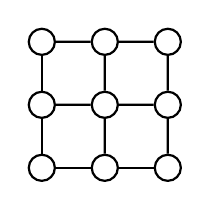
\begin{tikzpicture}[auto,
    specification/.style ={circle, draw, thick}, scale = 0.8]
   \node[specification] (A)  at (0,0)  {};
   \node[specification] (B)  at (1,0)  {};
   \node[specification] (C)  at (2,0)  {};
   \node[specification] (D)  at (0,1)  {};
   \node[specification] (E)  at (1,1)  {};
   \node[specification] (F)  at (2,1)  {};
   \node[specification] (G)  at (0,2)  {};
   \node[specification] (H)  at (1,2)  {};
   \node[specification] (I)  at (2,2)  {};

   \draw[thick] (A) to  (B);
   \draw[thick] (B) to  (C);
   \draw[thick] (D) to  (E);
   \draw[thick] (E) to  (F);
   \draw[thick] (G) to (H);
   \draw[thick] (H) to (I);
   \draw[thick] (A) to (D);
   \draw[thick] (B) to (E);
   \draw[thick] (C) to (F);
   \draw[thick] (D) to (G);
   \draw[thick] (E) to (H);
   \draw[thick] (F) to (I);
 \end{tikzpicture}
\end{minipage}\hfill
  B.
    \begin{minipage}{0.18\linewidth}
    \centering
    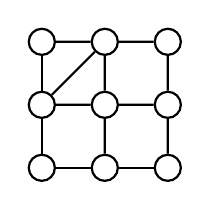
\begin{tikzpicture}[auto,
    specification/.style ={circle, draw, thick}, scale = 0.8]
   \node[specification] (A)  at (0,0)  {};
   \node[specification] (B)  at (1,0)  {};
   \node[specification] (C)  at (2,0)  {};
   \node[specification] (D)  at (0,1)  {};
   \node[specification] (E)  at (1,1)  {};
   \node[specification] (F)  at (2,1)  {};
   \node[specification] (G)  at (0,2)  {};
   \node[specification] (H)  at (1,2)  {};
   \node[specification] (I)  at (2,2)  {};

   \draw[thick] (A) to  (B);
   \draw[thick] (B) to  (C);
   \draw[thick] (D) to  (E);
   \draw[thick] (E) to  (F);
   \draw[thick] (G) to (H);
   \draw[thick] (H) to (I);
   \draw[thick] (A) to (D);
   \draw[thick] (B) to (E);
   \draw[thick] (C) to (F);
   \draw[thick] (D) to (G);
   \draw[thick] (E) to (H);
   \draw[thick] (F) to (I);
   \draw[thick] (D) to (H);

 \end{tikzpicture}
\end{minipage}\hfill
      C.
    \begin{minipage}{0.18\linewidth}
    \centering
    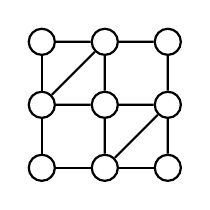
\begin{tikzpicture}[auto,
    specification/.style ={circle, draw, thick}, scale=0.8]
   \node[specification] (A)  at (0,0)  {};
   \node[specification] (B)  at (1,0)  {};
   \node[specification] (C)  at (2,0)  {};
   \node[specification] (D)  at (0,1)  {};
   \node[specification] (E)  at (1,1)  {};
   \node[specification] (F)  at (2,1)  {};
   \node[specification] (G)  at (0,2)  {};
   \node[specification] (H)  at (1,2)  {};
   \node[specification] (I)  at (2,2)  {};

   \draw[thick] (A) to  (B);
   \draw[thick] (B) to  (C);
   \draw[thick] (D) to  (E);
   \draw[thick] (E) to  (F);
   \draw[thick] (G) to (H);
   \draw[thick] (H) to (I);
   \draw[thick] (A) to (D);
   \draw[thick] (B) to (E);
   \draw[thick] (C) to (F);
   \draw[thick] (D) to (G);
   \draw[thick] (E) to (H);
   \draw[thick] (F) to (I);
   \draw[thick] (D) to (H);
   \draw[thick] (B) to (F);
 \end{tikzpicture}
\end{minipage}\hfill
      D.
    \begin{minipage}{0.18\linewidth}
    \centering
    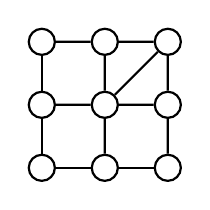
\begin{tikzpicture}[auto,
    specification/.style ={circle, draw, thick}, scale=0.8]
   \node[specification] (A)  at (0,0)  {};
   \node[specification] (B)  at (1,0)  {};
   \node[specification] (C)  at (2,0)  {};
   \node[specification] (D)  at (0,1)  {};
   \node[specification] (E)  at (1,1)  {};
   \node[specification] (F)  at (2,1)  {};
   \node[specification] (G)  at (0,2)  {};
   \node[specification] (H)  at (1,2)  {};
   \node[specification] (I)  at (2,2)  {};

   \draw[thick] (A) to  (B);
   \draw[thick] (B) to  (C);
   \draw[thick] (D) to  (E);
   \draw[thick] (E) to  (F);
   \draw[thick] (G) to (H);
   \draw[thick] (H) to (I);
   \draw[thick] (A) to (D);
   \draw[thick] (B) to (E);
   \draw[thick] (C) to (F);
   \draw[thick] (D) to (G);
   \draw[thick] (E) to (H);
   \draw[thick] (F) to (I);
   \draw[thick] (E) to (I);

 \end{tikzpicture}
\end{minipage}\hfill

\end{Ex}

\begin{Ex}
  以下4个图中,存在一条欧拉开迹的是$\underline{\quad\quad}$。
  \vspace{0.5cm}

  A.
    \begin{minipage}{0.18\linewidth}
    \centering
    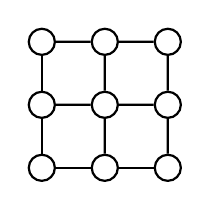
\begin{tikzpicture}[auto,
    specification/.style ={circle, draw, thick}, scale = 0.8]
   \node[specification] (A)  at (0,0)  {};
   \node[specification] (B)  at (1,0)  {};
   \node[specification] (C)  at (2,0)  {};
   \node[specification] (D)  at (0,1)  {};
   \node[specification] (E)  at (1,1)  {};
   \node[specification] (F)  at (2,1)  {};
   \node[specification] (G)  at (0,2)  {};
   \node[specification] (H)  at (1,2)  {};
   \node[specification] (I)  at (2,2)  {};

   \draw[thick] (A) to  (B);
   \draw[thick] (B) to  (C);
   \draw[thick] (D) to  (E);
   \draw[thick] (E) to  (F);
   \draw[thick] (G) to (H);
   \draw[thick] (H) to (I);
   \draw[thick] (A) to (D);
   \draw[thick] (B) to (E);
   \draw[thick] (C) to (F);
   \draw[thick] (D) to (G);
   \draw[thick] (E) to (H);
   \draw[thick] (F) to (I);
 \end{tikzpicture}
\end{minipage}\hfill
  B.
    \begin{minipage}{0.18\linewidth}
    \centering
    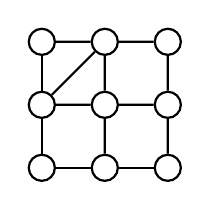
\begin{tikzpicture}[auto,
    specification/.style ={circle, draw, thick}, scale = 0.8]
   \node[specification] (A)  at (0,0)  {};
   \node[specification] (B)  at (1,0)  {};
   \node[specification] (C)  at (2,0)  {};
   \node[specification] (D)  at (0,1)  {};
   \node[specification] (E)  at (1,1)  {};
   \node[specification] (F)  at (2,1)  {};
   \node[specification] (G)  at (0,2)  {};
   \node[specification] (H)  at (1,2)  {};
   \node[specification] (I)  at (2,2)  {};

   \draw[thick] (A) to  (B);
   \draw[thick] (B) to  (C);
   \draw[thick] (D) to  (E);
   \draw[thick] (E) to  (F);
   \draw[thick] (G) to (H);
   \draw[thick] (H) to (I);
   \draw[thick] (A) to (D);
   \draw[thick] (B) to (E);
   \draw[thick] (C) to (F);
   \draw[thick] (D) to (G);
   \draw[thick] (E) to (H);
   \draw[thick] (F) to (I);
   \draw[thick] (D) to (H);

 \end{tikzpicture}
\end{minipage}\hfill
      C.
    \begin{minipage}{0.18\linewidth}
    \centering
    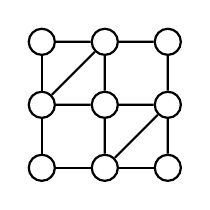
\begin{tikzpicture}[auto,
    specification/.style ={circle, draw, thick}, scale=0.8]
   \node[specification] (A)  at (0,0)  {};
   \node[specification] (B)  at (1,0)  {};
   \node[specification] (C)  at (2,0)  {};
   \node[specification] (D)  at (0,1)  {};
   \node[specification] (E)  at (1,1)  {};
   \node[specification] (F)  at (2,1)  {};
   \node[specification] (G)  at (0,2)  {};
   \node[specification] (H)  at (1,2)  {};
   \node[specification] (I)  at (2,2)  {};

   \draw[thick] (A) to  (B);
   \draw[thick] (B) to  (C);
   \draw[thick] (D) to  (E);
   \draw[thick] (E) to  (F);
   \draw[thick] (G) to (H);
   \draw[thick] (H) to (I);
   \draw[thick] (A) to (D);
   \draw[thick] (B) to (E);
   \draw[thick] (C) to (F);
   \draw[thick] (D) to (G);
   \draw[thick] (E) to (H);
   \draw[thick] (F) to (I);
   \draw[thick] (D) to (H);
   \draw[thick] (B) to (F);
 \end{tikzpicture}
\end{minipage}\hfill
      D.
    \begin{minipage}{0.18\linewidth}
    \centering
    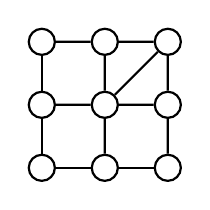
\begin{tikzpicture}[auto,
    specification/.style ={circle, draw, thick}, scale=0.8]
   \node[specification] (A)  at (0,0)  {};
   \node[specification] (B)  at (1,0)  {};
   \node[specification] (C)  at (2,0)  {};
   \node[specification] (D)  at (0,1)  {};
   \node[specification] (E)  at (1,1)  {};
   \node[specification] (F)  at (2,1)  {};
   \node[specification] (G)  at (0,2)  {};
   \node[specification] (H)  at (1,2)  {};
   \node[specification] (I)  at (2,2)  {};

   \draw[thick] (A) to  (B);
   \draw[thick] (B) to  (C);
   \draw[thick] (D) to  (E);
   \draw[thick] (E) to  (F);
   \draw[thick] (G) to (H);
   \draw[thick] (H) to (I);
   \draw[thick] (A) to (D);
   \draw[thick] (B) to (E);
   \draw[thick] (C) to (F);
   \draw[thick] (D) to (G);
   \draw[thick] (E) to (H);
   \draw[thick] (F) to (I);
   \draw[thick] (E) to (I);

 \end{tikzpicture}
\end{minipage}\hfill

\end{Ex}

\begin{Ex}
  以下4个图中,不可以一笔画成的是$\underline{\quad\quad}$。
  \vspace{0.5cm}

  A.
    \begin{minipage}{0.18\linewidth}
    \centering
    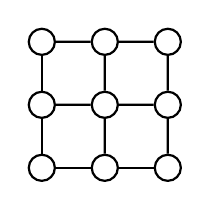
\begin{tikzpicture}[auto,
    specification/.style ={circle, draw, thick}, scale = 0.8]
   \node[specification] (A)  at (0,0)  {};
   \node[specification] (B)  at (1,0)  {};
   \node[specification] (C)  at (2,0)  {};
   \node[specification] (D)  at (0,1)  {};
   \node[specification] (E)  at (1,1)  {};
   \node[specification] (F)  at (2,1)  {};
   \node[specification] (G)  at (0,2)  {};
   \node[specification] (H)  at (1,2)  {};
   \node[specification] (I)  at (2,2)  {};

   \draw[thick] (A) to  (B);
   \draw[thick] (B) to  (C);
   \draw[thick] (D) to  (E);
   \draw[thick] (E) to  (F);
   \draw[thick] (G) to (H);
   \draw[thick] (H) to (I);
   \draw[thick] (A) to (D);
   \draw[thick] (B) to (E);
   \draw[thick] (C) to (F);
   \draw[thick] (D) to (G);
   \draw[thick] (E) to (H);
   \draw[thick] (F) to (I);
 \end{tikzpicture}
\end{minipage}\hfill
  B.
    \begin{minipage}{0.18\linewidth}
    \centering
    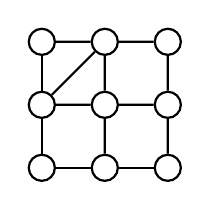
\begin{tikzpicture}[auto,
    specification/.style ={circle, draw, thick}, scale = 0.8]
   \node[specification] (A)  at (0,0)  {};
   \node[specification] (B)  at (1,0)  {};
   \node[specification] (C)  at (2,0)  {};
   \node[specification] (D)  at (0,1)  {};
   \node[specification] (E)  at (1,1)  {};
   \node[specification] (F)  at (2,1)  {};
   \node[specification] (G)  at (0,2)  {};
   \node[specification] (H)  at (1,2)  {};
   \node[specification] (I)  at (2,2)  {};

   \draw[thick] (A) to  (B);
   \draw[thick] (B) to  (C);
   \draw[thick] (D) to  (E);
   \draw[thick] (E) to  (F);
   \draw[thick] (G) to (H);
   \draw[thick] (H) to (I);
   \draw[thick] (A) to (D);
   \draw[thick] (B) to (E);
   \draw[thick] (C) to (F);
   \draw[thick] (D) to (G);
   \draw[thick] (E) to (H);
   \draw[thick] (F) to (I);
   \draw[thick] (D) to (H);

 \end{tikzpicture}
\end{minipage}\hfill
      C.
    \begin{minipage}{0.18\linewidth}
    \centering
    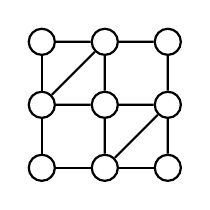
\begin{tikzpicture}[auto,
    specification/.style ={circle, draw, thick}, scale=0.8]
   \node[specification] (A)  at (0,0)  {};
   \node[specification] (B)  at (1,0)  {};
   \node[specification] (C)  at (2,0)  {};
   \node[specification] (D)  at (0,1)  {};
   \node[specification] (E)  at (1,1)  {};
   \node[specification] (F)  at (2,1)  {};
   \node[specification] (G)  at (0,2)  {};
   \node[specification] (H)  at (1,2)  {};
   \node[specification] (I)  at (2,2)  {};

   \draw[thick] (A) to  (B);
   \draw[thick] (B) to  (C);
   \draw[thick] (D) to  (E);
   \draw[thick] (E) to  (F);
   \draw[thick] (G) to (H);
   \draw[thick] (H) to (I);
   \draw[thick] (A) to (D);
   \draw[thick] (B) to (E);
   \draw[thick] (C) to (F);
   \draw[thick] (D) to (G);
   \draw[thick] (E) to (H);
   \draw[thick] (F) to (I);
   \draw[thick] (D) to (H);
   \draw[thick] (B) to (F);
 \end{tikzpicture}
\end{minipage}\hfill
      D.
    \begin{minipage}{0.18\linewidth}
    \centering
    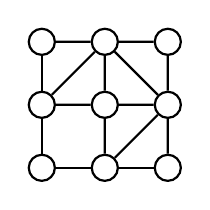
\begin{tikzpicture}[auto,
    specification/.style ={circle, draw, thick}, scale=0.8]
   \node[specification] (A)  at (0,0)  {};
   \node[specification] (B)  at (1,0)  {};
   \node[specification] (C)  at (2,0)  {};
   \node[specification] (D)  at (0,1)  {};
   \node[specification] (E)  at (1,1)  {};
   \node[specification] (F)  at (2,1)  {};
   \node[specification] (G)  at (0,2)  {};
   \node[specification] (H)  at (1,2)  {};
   \node[specification] (I)  at (2,2)  {};

   \draw[thick] (A) to  (B);
   \draw[thick] (B) to  (C);
   \draw[thick] (D) to  (E);
   \draw[thick] (E) to  (F);
   \draw[thick] (G) to (H);
   \draw[thick] (H) to (I);
   \draw[thick] (A) to (D);
   \draw[thick] (B) to (E);
   \draw[thick] (C) to (F);
   \draw[thick] (D) to (G);
   \draw[thick] (E) to (H);
   \draw[thick] (F) to (I);
   \draw[thick] (D) to (H);
   \draw[thick] (B) to (F);
   \draw[thick] (H) to (F);

 \end{tikzpicture}
\end{minipage}\hfill


\end{Ex}


\begin{Ex}
  以下4个图中,至少需要两笔才能画成的是$\underline{\quad\quad}$。
  \vspace{0.5cm}

  A.
    \begin{minipage}{0.18\linewidth}
    \centering
    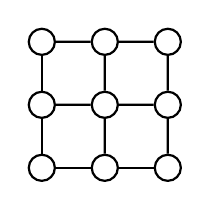
\begin{tikzpicture}[auto,
    specification/.style ={circle, draw, thick}, scale = 0.8]
   \node[specification] (A)  at (0,0)  {};
   \node[specification] (B)  at (1,0)  {};
   \node[specification] (C)  at (2,0)  {};
   \node[specification] (D)  at (0,1)  {};
   \node[specification] (E)  at (1,1)  {};
   \node[specification] (F)  at (2,1)  {};
   \node[specification] (G)  at (0,2)  {};
   \node[specification] (H)  at (1,2)  {};
   \node[specification] (I)  at (2,2)  {};

   \draw[thick] (A) to  (B);
   \draw[thick] (B) to  (C);
   \draw[thick] (D) to  (E);
   \draw[thick] (E) to  (F);
   \draw[thick] (G) to (H);
   \draw[thick] (H) to (I);
   \draw[thick] (A) to (D);
   \draw[thick] (B) to (E);
   \draw[thick] (C) to (F);
   \draw[thick] (D) to (G);
   \draw[thick] (E) to (H);
   \draw[thick] (F) to (I);
 \end{tikzpicture}
\end{minipage}\hfill
  B.
    \begin{minipage}{0.18\linewidth}
    \centering
    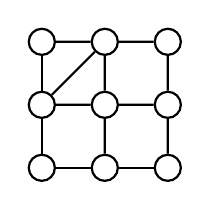
\begin{tikzpicture}[auto,
    specification/.style ={circle, draw, thick}, scale = 0.8]
   \node[specification] (A)  at (0,0)  {};
   \node[specification] (B)  at (1,0)  {};
   \node[specification] (C)  at (2,0)  {};
   \node[specification] (D)  at (0,1)  {};
   \node[specification] (E)  at (1,1)  {};
   \node[specification] (F)  at (2,1)  {};
   \node[specification] (G)  at (0,2)  {};
   \node[specification] (H)  at (1,2)  {};
   \node[specification] (I)  at (2,2)  {};

   \draw[thick] (A) to  (B);
   \draw[thick] (B) to  (C);
   \draw[thick] (D) to  (E);
   \draw[thick] (E) to  (F);
   \draw[thick] (G) to (H);
   \draw[thick] (H) to (I);
   \draw[thick] (A) to (D);
   \draw[thick] (B) to (E);
   \draw[thick] (C) to (F);
   \draw[thick] (D) to (G);
   \draw[thick] (E) to (H);
   \draw[thick] (F) to (I);
   \draw[thick] (D) to (H);

 \end{tikzpicture}
\end{minipage}\hfill
      C.
    \begin{minipage}{0.18\linewidth}
    \centering
    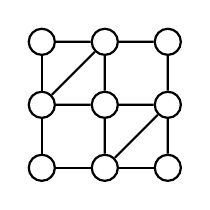
\begin{tikzpicture}[auto,
    specification/.style ={circle, draw, thick}, scale=0.8]
   \node[specification] (A)  at (0,0)  {};
   \node[specification] (B)  at (1,0)  {};
   \node[specification] (C)  at (2,0)  {};
   \node[specification] (D)  at (0,1)  {};
   \node[specification] (E)  at (1,1)  {};
   \node[specification] (F)  at (2,1)  {};
   \node[specification] (G)  at (0,2)  {};
   \node[specification] (H)  at (1,2)  {};
   \node[specification] (I)  at (2,2)  {};

   \draw[thick] (A) to  (B);
   \draw[thick] (B) to  (C);
   \draw[thick] (D) to  (E);
   \draw[thick] (E) to  (F);
   \draw[thick] (G) to (H);
   \draw[thick] (H) to (I);
   \draw[thick] (A) to (D);
   \draw[thick] (B) to (E);
   \draw[thick] (C) to (F);
   \draw[thick] (D) to (G);
   \draw[thick] (E) to (H);
   \draw[thick] (F) to (I);
   \draw[thick] (D) to (H);
   \draw[thick] (B) to (F);
 \end{tikzpicture}
\end{minipage}\hfill
      D.
    \begin{minipage}{0.18\linewidth}
    \centering
    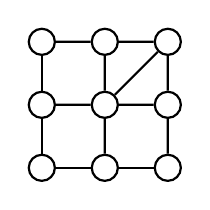
\begin{tikzpicture}[auto,
    specification/.style ={circle, draw, thick}, scale=0.8]
   \node[specification] (A)  at (0,0)  {};
   \node[specification] (B)  at (1,0)  {};
   \node[specification] (C)  at (2,0)  {};
   \node[specification] (D)  at (0,1)  {};
   \node[specification] (E)  at (1,1)  {};
   \node[specification] (F)  at (2,1)  {};
   \node[specification] (G)  at (0,2)  {};
   \node[specification] (H)  at (1,2)  {};
   \node[specification] (I)  at (2,2)  {};

   \draw[thick] (A) to  (B);
   \draw[thick] (B) to  (C);
   \draw[thick] (D) to  (E);
   \draw[thick] (E) to  (F);
   \draw[thick] (G) to (H);
   \draw[thick] (H) to (I);
   \draw[thick] (A) to (D);
   \draw[thick] (B) to (E);
   \draw[thick] (C) to (F);
   \draw[thick] (D) to (G);
   \draw[thick] (E) to (H);
   \draw[thick] (F) to (I);
   \draw[thick] (E) to (I);

 \end{tikzpicture}
\end{minipage}\hfill

\end{Ex}


\begin{Ex}
  以下4个图中,至少需要三笔才能画成的是$\underline{\quad\quad}$。
  \vspace{0.5cm}

  A.
    \begin{minipage}{0.18\linewidth}
    \centering
    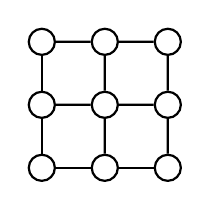
\begin{tikzpicture}[auto,
    specification/.style ={circle, draw, thick}, scale = 0.8]
   \node[specification] (A)  at (0,0)  {};
   \node[specification] (B)  at (1,0)  {};
   \node[specification] (C)  at (2,0)  {};
   \node[specification] (D)  at (0,1)  {};
   \node[specification] (E)  at (1,1)  {};
   \node[specification] (F)  at (2,1)  {};
   \node[specification] (G)  at (0,2)  {};
   \node[specification] (H)  at (1,2)  {};
   \node[specification] (I)  at (2,2)  {};

   \draw[thick] (A) to  (B);
   \draw[thick] (B) to  (C);
   \draw[thick] (D) to  (E);
   \draw[thick] (E) to  (F);
   \draw[thick] (G) to (H);
   \draw[thick] (H) to (I);
   \draw[thick] (A) to (D);
   \draw[thick] (B) to (E);
   \draw[thick] (C) to (F);
   \draw[thick] (D) to (G);
   \draw[thick] (E) to (H);
   \draw[thick] (F) to (I);
 \end{tikzpicture}
\end{minipage}\hfill
  B.
    \begin{minipage}{0.18\linewidth}
    \centering
    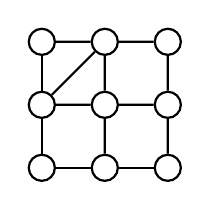
\begin{tikzpicture}[auto,
    specification/.style ={circle, draw, thick}, scale = 0.8]
   \node[specification] (A)  at (0,0)  {};
   \node[specification] (B)  at (1,0)  {};
   \node[specification] (C)  at (2,0)  {};
   \node[specification] (D)  at (0,1)  {};
   \node[specification] (E)  at (1,1)  {};
   \node[specification] (F)  at (2,1)  {};
   \node[specification] (G)  at (0,2)  {};
   \node[specification] (H)  at (1,2)  {};
   \node[specification] (I)  at (2,2)  {};

   \draw[thick] (A) to  (B);
   \draw[thick] (B) to  (C);
   \draw[thick] (D) to  (E);
   \draw[thick] (E) to  (F);
   \draw[thick] (G) to (H);
   \draw[thick] (H) to (I);
   \draw[thick] (A) to (D);
   \draw[thick] (B) to (E);
   \draw[thick] (C) to (F);
   \draw[thick] (D) to (G);
   \draw[thick] (E) to (H);
   \draw[thick] (F) to (I);
   \draw[thick] (D) to (H);

 \end{tikzpicture}
\end{minipage}\hfill
      C.
    \begin{minipage}{0.18\linewidth}
    \centering
    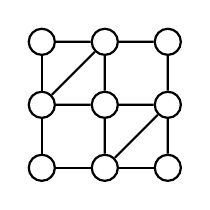
\begin{tikzpicture}[auto,
    specification/.style ={circle, draw, thick}, scale=0.8]
   \node[specification] (A)  at (0,0)  {};
   \node[specification] (B)  at (1,0)  {};
   \node[specification] (C)  at (2,0)  {};
   \node[specification] (D)  at (0,1)  {};
   \node[specification] (E)  at (1,1)  {};
   \node[specification] (F)  at (2,1)  {};
   \node[specification] (G)  at (0,2)  {};
   \node[specification] (H)  at (1,2)  {};
   \node[specification] (I)  at (2,2)  {};

   \draw[thick] (A) to  (B);
   \draw[thick] (B) to  (C);
   \draw[thick] (D) to  (E);
   \draw[thick] (E) to  (F);
   \draw[thick] (G) to (H);
   \draw[thick] (H) to (I);
   \draw[thick] (A) to (D);
   \draw[thick] (B) to (E);
   \draw[thick] (C) to (F);
   \draw[thick] (D) to (G);
   \draw[thick] (E) to (H);
   \draw[thick] (F) to (I);
   \draw[thick] (D) to (H);
   \draw[thick] (B) to (F);
 \end{tikzpicture}
\end{minipage}\hfill
      D.
    \begin{minipage}{0.18\linewidth}
    \centering
    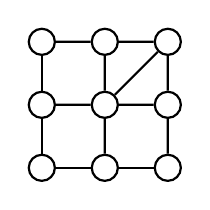
\begin{tikzpicture}[auto,
    specification/.style ={circle, draw, thick}, scale=0.8]
   \node[specification] (A)  at (0,0)  {};
   \node[specification] (B)  at (1,0)  {};
   \node[specification] (C)  at (2,0)  {};
   \node[specification] (D)  at (0,1)  {};
   \node[specification] (E)  at (1,1)  {};
   \node[specification] (F)  at (2,1)  {};
   \node[specification] (G)  at (0,2)  {};
   \node[specification] (H)  at (1,2)  {};
   \node[specification] (I)  at (2,2)  {};

   \draw[thick] (A) to  (B);
   \draw[thick] (B) to  (C);
   \draw[thick] (D) to  (E);
   \draw[thick] (E) to  (F);
   \draw[thick] (G) to (H);
   \draw[thick] (H) to (I);
   \draw[thick] (A) to (D);
   \draw[thick] (B) to (E);
   \draw[thick] (C) to (F);
   \draw[thick] (D) to (G);
   \draw[thick] (E) to (H);
   \draw[thick] (F) to (I);
   \draw[thick] (E) to (I);

 \end{tikzpicture}
\end{minipage}\hfill

\end{Ex}

  \chapter{哈密顿图}

若图$G$含有一条包含所有结点的路,则将其称之为图$G$的一条{\bfseries 哈密顿路}。
若图$G$含有一个包含所有结点的圈,则将其称之为图$G$的一个{\bfseries哈密顿圈}。包
含哈密顿圈的图称之为{\bfseries 哈密顿图}。



\begin{Ex}
  下图是否是哈密顿图?若是,找出一个哈密顿圈?若不是,说明理由。

\centering  
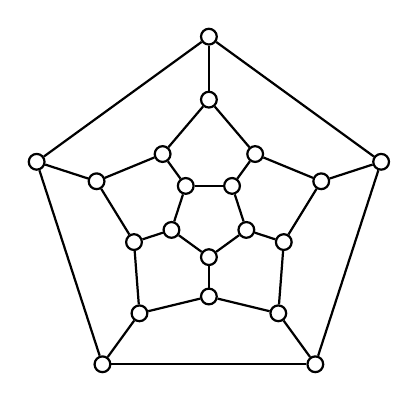
\begin{tikzpicture}[auto,
    specification/.style ={circle, draw, thick, inner sep = 0pt, minimum size=2mm}]
   \node[specification] (A)  at (18:2.3cm)  {};
   \node[specification] (B)  at (90:2.3cm)  {};
   \node[specification] (C)  at (162:2.3cm)  {};
   \node[specification] (D) at (234:2.3cm)  {};
   \node[specification] (E)  at (306:2.3cm)  {};
   \node[specification] (F)  at (18:1.5cm)  {};
   \node[specification] (G)  at (90:1.5cm)  {};
   \node[specification] (H)  at (162:1.5cm)  {};
   \node[specification] (I) at (234:1.5cm)  {};
   \node[specification] (J)  at (306:1.5cm)  {};
   \node[specification] (K)  at (-18:1.0cm)  {};
   \node[specification] (L)  at (-90:1.0cm)  {};
   \node[specification] (M)  at (-162:1.0cm)  {};
   \node[specification] (N) at (-234:1.0cm)  {};
   \node[specification] (O)  at (-306:1.0cm)  {};
   \node[specification] (P)  at (-18:0.5cm)  {};
   \node[specification] (Q)  at (-90:0.5cm)  {};
   \node[specification] (R)  at (-162:0.5cm)  {};
   \node[specification] (S) at (-234:0.5cm)  {};
   \node[specification] (T)  at (-306:0.5cm)  {};
   
   
   \draw[thick] (A) to  (B);
   \draw[thick] (B) to  (C);
   \draw[thick] (C) to  (D);
   \draw[thick] (D) to  (E);
   \draw[thick] (E) to  (A);
   \draw[thick] (A) to  (F);
   \draw[thick] (B) to  (G);
   \draw[thick] (C) to  (H);
   \draw[thick] (D) to  (I);
   \draw[thick] (E) to  (J);

   \draw[thick] (F) to  (O);
   \draw[thick] (O) to  (G);
   \draw[thick] (G) to  (N);
   \draw[thick] (N) to  (H);
   \draw[thick] (H) to  (M);
   \draw[thick] (M) to  (I);
   \draw[thick] (I) to  (L);
   \draw[thick] (L) to  (J);
   \draw[thick] (J) to  (K);
   \draw[thick] (K) to  (F);

   \draw[thick] (P) to  (K);
   \draw[thick] (Q) to  (L);
   \draw[thick] (R) to  (M);
   \draw[thick] (S) to  (N);
   \draw[thick] (T) to  (O);

   \draw[thick] (P) to  (Q);
   \draw[thick] (Q) to  (R);
   \draw[thick] (R) to  (S);
   \draw[thick] (S) to  (T);
   \draw[thick] (T) to  (P);
 \end{tikzpicture}
\end{Ex}


\begin{Ex}
  下图是否是哈密顿图?若是,找出一个哈密顿圈?若不是,说明理由。

  \centering
  
      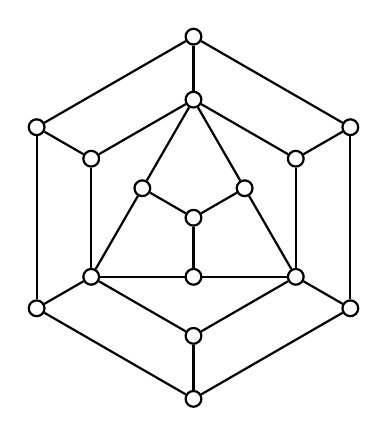
\begin{tikzpicture}[auto,
    specification/.style ={circle, draw, thick, inner sep = 0pt, minimum size=2mm}]
   \node[specification] (A)  at (30:2.3cm)  {};
   \node[specification] (B)  at (90:2.3cm)  {};
   \node[specification] (C)  at (150:2.3cm)  {};
   \node[specification] (D) at (210:2.3cm)  {};
   \node[specification] (E)  at (270:2.3cm)  {};
   \node[specification] (F)  at (330:2.3cm)  {};
   \node[specification] (G)  at (30:1.5cm)  {};
   \node[specification] (H)  at (90:1.5cm)  {};
   \node[specification] (I) at (150:1.5cm)  {};
   \node[specification] (J)  at (210:1.5cm)  {};
   \node[specification] (K)  at (270:1.5cm)  {};
   \node[specification] (L)  at (330:1.5cm)  {};
   \node[specification] (M)  at (30:0.75cm)  {};
   \node[specification] (N)  at (150:0.75cm)  {};
   \node[specification] (P)  at (270:0.75cm)  {};
   \node[specification] (Q)  at (0,0)  {};
   \draw[thick] (A) to  (B);
   \draw[thick] (B) to  (C);
   \draw[thick] (C) to  (D);
   \draw[thick] (D) to  (E);
   \draw[thick] (E) to  (F);
   \draw[thick] (F) to  (A);
   \draw[thick] (A) to  (G);
   \draw[thick] (B) to  (H);
   \draw[thick] (C) to  (I);
   \draw[thick] (D) to  (J);
   \draw[thick] (E) to  (K);
   \draw[thick] (F) to  (L);
   \draw[thick] (G) to  (H);
   \draw[thick] (H) to  (I);
   \draw[thick] (I) to  (J);
   \draw[thick] (J) to  (K);
   \draw[thick] (K) to  (L);
   \draw[thick] (L) to  (G);
   \draw[thick] (H) to  (M);
   \draw[thick] (M) to  (L);
   \draw[thick] (L) to  (P);
   \draw[thick] (P) to  (J);
   \draw[thick] (J) to  (N);
   \draw[thick] (N) to  (H);
   \draw[thick] (M) to  (Q);
   \draw[thick] (N) to  (Q);
   \draw[thick] (P) to  (Q);
 \end{tikzpicture}

\end{Ex}
\begin{Ex}
  下图是否是哈密顿图?若是,找出一个哈密顿圈?若不是,说明理由。

  \centering
  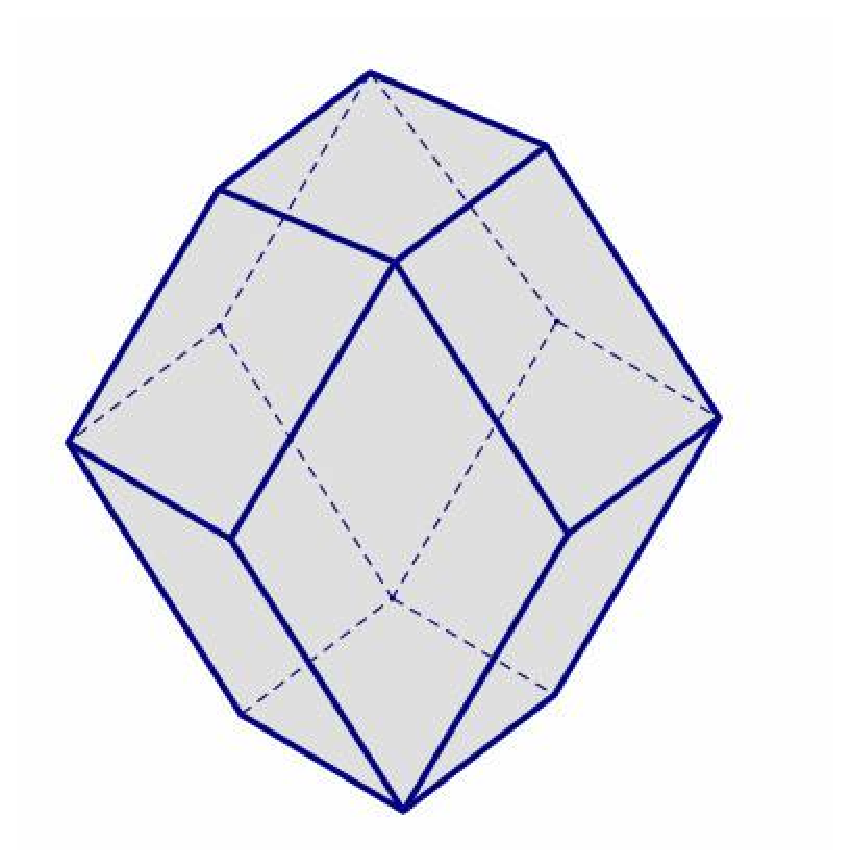
\includegraphics[width=5cm,height=4cm]{timg}

\end{Ex}

\begin{Ex}
  下图是否是哈密顿图?若是,找出一个哈密顿圈?若不是,说明理由。

  \centering
      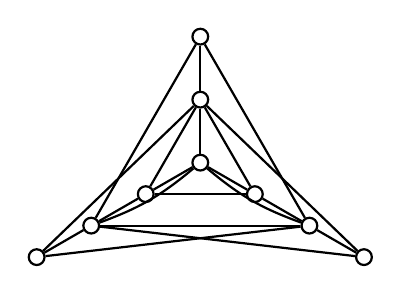
\begin{tikzpicture}[auto,
    specification/.style ={circle, draw, thick, inner sep = 0pt, minimum size=2mm}]
   \node[specification] (A)  at (90:1.6cm)  {};
   \node[specification] (B)  at (210:1.6cm)  {};
   \node[specification] (C)  at (330:1.6cm)  {};
   \node[specification] (D)  at (90:0.8cm)  {};
   \node[specification] (E)  at (210:0.8cm)  {};
   \node[specification] (F)  at (330:0.8cm)  {};
   \node[specification] (G)  at (210:2.4cm)  {};
   \node[specification] (H)  at (330:2.4cm)  {};
   \node[specification] (I)  at (0,0)  {};
   
   
   \draw[thick] (A) to  (B);
   \draw[thick] (B) to  (C);
   \draw[thick] (C) to  (A);
   \draw[thick] (D) to  (E);
   \draw[thick] (E) to  (F);
   \draw[thick] (F) to  (D);
   \draw[thick] (D) to  (G);
   \draw[thick] (D) to  (H);
   \draw[thick] (H) to  (B);
   \draw[thick] (G) to  (C);
   \draw[thick] (A) to  (D);
   \draw[thick] (C) to  (F);
   \draw[thick] (B) to  (E);
   \draw[thick] (I) to  (D);
   \draw[thick] (I) to  (E);
   \draw[thick] (I) to  (F);
   \draw[thick] (G) to  (B);
   \draw[thick] (H) to  (C);
   \draw[thick] (B) to [bend right = 10] (I);
   \draw[thick] (C) to [bend left = 10] (I);
 \end{tikzpicture}


\end{Ex}


\begin{Ex}
  下图是否是哈密顿图?若是,找出一个哈密顿圈?若不是,说明理由。

\centering  
      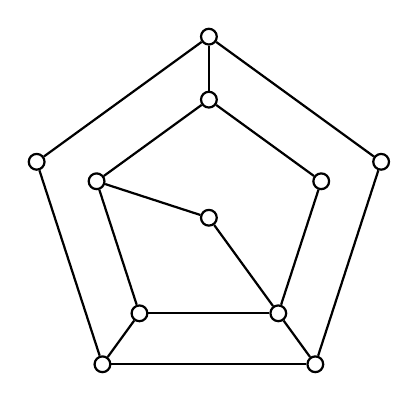
\begin{tikzpicture}[auto,
    specification/.style ={circle, draw, thick, inner sep = 0pt, minimum size=2mm}]
   \node[specification] (A)  at (18:2.3cm)  {};
   \node[specification] (B)  at (90:2.3cm)  {};
   \node[specification] (C)  at (162:2.3cm)  {};
   \node[specification] (D) at (234:2.3cm)  {};
   \node[specification] (E)  at (306:2.3cm)  {};
   \node[specification] (F)  at (18:1.5cm)  {};
   \node[specification] (G)  at (90:1.5cm)  {};
   \node[specification] (H)  at (162:1.5cm)  {};
   \node[specification] (I) at (234:1.5cm)  {};
   \node[specification] (J)  at (306:1.5cm)  {};
   \node[specification] (K)  at (0,0)  {};
   
   
   
   \draw[thick] (A) to  (B);
   \draw[thick] (B) to  (C);
   \draw[thick] (C) to  (D);
   \draw[thick] (D) to  (E);
   \draw[thick] (E) to  (A);
   
   \draw[thick] (F) to  (G);
   \draw[thick] (G) to  (H);
   \draw[thick] (H) to  (I);
   \draw[thick] (I) to  (J);
   \draw[thick] (J) to  (F);
   
   \draw[thick] (B) to  (G);
   \draw[thick] (D) to  (I);
   \draw[thick] (E) to  (J);
   \draw[thick] (K) to  (H);
   \draw[thick] (K) to  (J);

 \end{tikzpicture}
\end{Ex}

\begin{Ex}
  下图是否是哈密顿图?若是,找出一个哈密顿圈?若不是,说明理由。

  \centering
      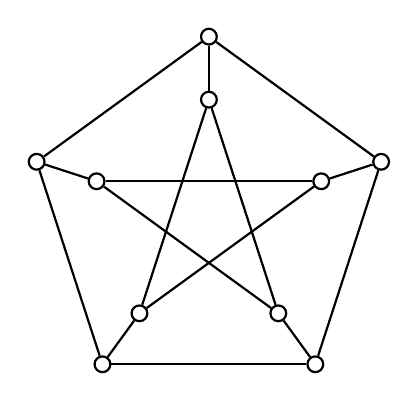
\begin{tikzpicture}[auto,
    specification/.style ={circle, draw, thick, inner sep = 0pt, minimum size=2mm}]
   \node[specification] (A)  at (18:2.3cm)  {};
   \node[specification] (B)  at (90:2.3cm)  {};
   \node[specification] (C)  at (162:2.3cm)  {};
   \node[specification] (D) at (234:2.3cm)  {};
   \node[specification] (E)  at (306:2.3cm)  {};
   \node[specification] (F)  at (18:1.5cm)  {};
   \node[specification] (G)  at (90:1.5cm)  {};
   \node[specification] (H)  at (162:1.5cm)  {};
   \node[specification] (I) at (234:1.5cm)  {};
   \node[specification] (J)  at (306:1.5cm)  {};
   
   
   \draw[thick] (A) to  (B);
   \draw[thick] (B) to  (C);
   \draw[thick] (C) to  (D);
   \draw[thick] (D) to  (E);
   \draw[thick] (E) to  (A);
   \draw[thick] (A) to  (F);
   \draw[thick] (B) to  (G);
   \draw[thick] (C) to  (H);
   \draw[thick] (D) to  (I);
   \draw[thick] (E) to  (J);
   \draw[thick] (G) to  (I);
   \draw[thick] (I) to  (F);
   \draw[thick] (F) to  (H);
   \draw[thick] (H) to  (J);
   \draw[thick] (J) to  (G);

 \end{tikzpicture}
\end{Ex}


\begin{Ex}
  以下4个图中,存在一个哈密顿圈的是$\underline{\quad\quad}$。
  \vspace{0.5cm}

  A.
    \begin{minipage}{0.18\linewidth}
    \centering
    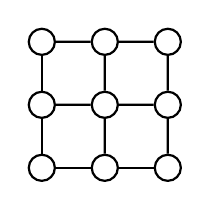
\begin{tikzpicture}[auto,
    specification/.style ={circle, draw, thick}, scale = 0.8]
   \node[specification] (A)  at (0,0)  {};
   \node[specification] (B)  at (1,0)  {};
   \node[specification] (C)  at (2,0)  {};
   \node[specification] (D)  at (0,1)  {};
   \node[specification] (E)  at (1,1)  {};
   \node[specification] (F)  at (2,1)  {};
   \node[specification] (G)  at (0,2)  {};
   \node[specification] (H)  at (1,2)  {};
   \node[specification] (I)  at (2,2)  {};

   \draw[thick] (A) to  (B);
   \draw[thick] (B) to  (C);
   \draw[thick] (D) to  (E);
   \draw[thick] (E) to  (F);
   \draw[thick] (G) to (H);
   \draw[thick] (H) to (I);
   \draw[thick] (A) to (D);
   \draw[thick] (B) to (E);
   \draw[thick] (C) to (F);
   \draw[thick] (D) to (G);
   \draw[thick] (E) to (H);
   \draw[thick] (F) to (I);
 \end{tikzpicture}
\end{minipage}\hfill
  B.
    \begin{minipage}{0.18\linewidth}
    \centering
    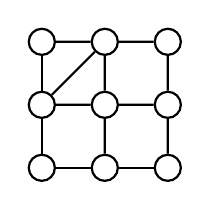
\begin{tikzpicture}[auto,
    specification/.style ={circle, draw, thick}, scale = 0.8]
   \node[specification] (A)  at (0,0)  {};
   \node[specification] (B)  at (1,0)  {};
   \node[specification] (C)  at (2,0)  {};
   \node[specification] (D)  at (0,1)  {};
   \node[specification] (E)  at (1,1)  {};
   \node[specification] (F)  at (2,1)  {};
   \node[specification] (G)  at (0,2)  {};
   \node[specification] (H)  at (1,2)  {};
   \node[specification] (I)  at (2,2)  {};

   \draw[thick] (A) to  (B);
   \draw[thick] (B) to  (C);
   \draw[thick] (D) to  (E);
   \draw[thick] (E) to  (F);
   \draw[thick] (G) to (H);
   \draw[thick] (H) to (I);
   \draw[thick] (A) to (D);
   \draw[thick] (B) to (E);
   \draw[thick] (C) to (F);
   \draw[thick] (D) to (G);
   \draw[thick] (E) to (H);
   \draw[thick] (F) to (I);
   \draw[thick] (D) to (H);

 \end{tikzpicture}
\end{minipage}\hfill
      C.
    \begin{minipage}{0.18\linewidth}
    \centering
    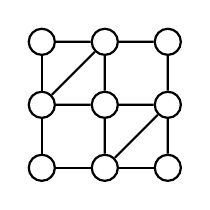
\begin{tikzpicture}[auto,
    specification/.style ={circle, draw, thick}, scale=0.8]
   \node[specification] (A)  at (0,0)  {};
   \node[specification] (B)  at (1,0)  {};
   \node[specification] (C)  at (2,0)  {};
   \node[specification] (D)  at (0,1)  {};
   \node[specification] (E)  at (1,1)  {};
   \node[specification] (F)  at (2,1)  {};
   \node[specification] (G)  at (0,2)  {};
   \node[specification] (H)  at (1,2)  {};
   \node[specification] (I)  at (2,2)  {};

   \draw[thick] (A) to  (B);
   \draw[thick] (B) to  (C);
   \draw[thick] (D) to  (E);
   \draw[thick] (E) to  (F);
   \draw[thick] (G) to (H);
   \draw[thick] (H) to (I);
   \draw[thick] (A) to (D);
   \draw[thick] (B) to (E);
   \draw[thick] (C) to (F);
   \draw[thick] (D) to (G);
   \draw[thick] (E) to (H);
   \draw[thick] (F) to (I);
   \draw[thick] (D) to (H);
   \draw[thick] (B) to (F);
 \end{tikzpicture}
\end{minipage}\hfill
      D.
    \begin{minipage}{0.18\linewidth}
    \centering
    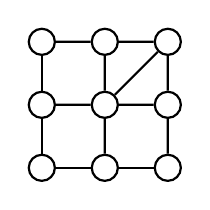
\begin{tikzpicture}[auto,
    specification/.style ={circle, draw, thick}, scale=0.8]
   \node[specification] (A)  at (0,0)  {};
   \node[specification] (B)  at (1,0)  {};
   \node[specification] (C)  at (2,0)  {};
   \node[specification] (D)  at (0,1)  {};
   \node[specification] (E)  at (1,1)  {};
   \node[specification] (F)  at (2,1)  {};
   \node[specification] (G)  at (0,2)  {};
   \node[specification] (H)  at (1,2)  {};
   \node[specification] (I)  at (2,2)  {};

   \draw[thick] (A) to  (B);
   \draw[thick] (B) to  (C);
   \draw[thick] (D) to  (E);
   \draw[thick] (E) to  (F);
   \draw[thick] (G) to (H);
   \draw[thick] (H) to (I);
   \draw[thick] (A) to (D);
   \draw[thick] (B) to (E);
   \draw[thick] (C) to (F);
   \draw[thick] (D) to (G);
   \draw[thick] (E) to (H);
   \draw[thick] (F) to (I);
   \draw[thick] (E) to (I);

 \end{tikzpicture}
\end{minipage}\hfill

\end{Ex}

\begin{Ex}
  以下4个图中,不存在哈密顿路的是$\underline{\quad\quad}$。
  \vspace{0.5cm}

  A.
    \begin{minipage}{0.18\linewidth}
    \centering
    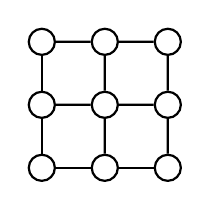
\begin{tikzpicture}[auto,
    specification/.style ={circle, draw, thick}, scale = 0.8]
   \node[specification] (A)  at (0,0)  {};
   \node[specification] (B)  at (1,0)  {};
   \node[specification] (C)  at (2,0)  {};
   \node[specification] (D)  at (0,1)  {};
   \node[specification] (E)  at (1,1)  {};
   \node[specification] (F)  at (2,1)  {};
   \node[specification] (G)  at (0,2)  {};
   \node[specification] (H)  at (1,2)  {};
   \node[specification] (I)  at (2,2)  {};

   \draw[thick] (A) to  (B);
   \draw[thick] (B) to  (C);
   \draw[thick] (D) to  (E);
   \draw[thick] (E) to  (F);
   \draw[thick] (G) to (H);
   \draw[thick] (H) to (I);
   \draw[thick] (A) to (D);
   \draw[thick] (B) to (E);
   \draw[thick] (C) to (F);
   \draw[thick] (D) to (G);
   \draw[thick] (E) to (H);
   \draw[thick] (F) to (I);
 \end{tikzpicture}
\end{minipage}\hfill
  B.
    \begin{minipage}{0.18\linewidth}
    \centering
    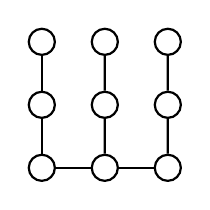
\begin{tikzpicture}[auto,
    specification/.style ={circle, draw, thick}, scale = 0.8]
   \node[specification] (A)  at (0,0)  {};
   \node[specification] (B)  at (1,0)  {};
   \node[specification] (C)  at (2,0)  {};
   \node[specification] (D)  at (0,1)  {};
   \node[specification] (E)  at (1,1)  {};
   \node[specification] (F)  at (2,1)  {};
   \node[specification] (G)  at (0,2)  {};
   \node[specification] (H)  at (1,2)  {};
   \node[specification] (I)  at (2,2)  {};

   \draw[thick] (A) to  (B);
   \draw[thick] (B) to  (C);
   \draw[thick] (A) to (D);
   \draw[thick] (B) to (E);
   \draw[thick] (C) to (F);
   \draw[thick] (D) to (G);
   \draw[thick] (E) to (H);
   \draw[thick] (F) to (I);

 \end{tikzpicture}
\end{minipage}\hfill
      C.
    \begin{minipage}{0.18\linewidth}
    \centering
    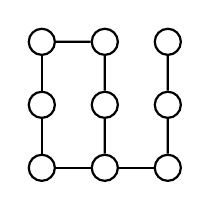
\begin{tikzpicture}[auto,
    specification/.style ={circle, draw, thick}, scale=0.8]
   \node[specification] (A)  at (0,0)  {};
   \node[specification] (B)  at (1,0)  {};
   \node[specification] (C)  at (2,0)  {};
   \node[specification] (D)  at (0,1)  {};
   \node[specification] (E)  at (1,1)  {};
   \node[specification] (F)  at (2,1)  {};
   \node[specification] (G)  at (0,2)  {};
   \node[specification] (H)  at (1,2)  {};
   \node[specification] (I)  at (2,2)  {};

   \draw[thick] (A) to  (B);
   \draw[thick] (B) to  (C);
   \draw[thick] (A) to (D);
   \draw[thick] (B) to (E);
   \draw[thick] (C) to (F);
   \draw[thick] (D) to (G);
   \draw[thick] (E) to (H);
   \draw[thick] (F) to (I);
   \draw[thick] (G) to (H);
 \end{tikzpicture}
\end{minipage}\hfill
      D.
    \begin{minipage}{0.18\linewidth}
    \centering
    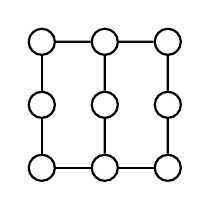
\begin{tikzpicture}[auto,
    specification/.style ={circle, draw, thick}, scale=0.8]
   \node[specification] (A)  at (0,0)  {};
   \node[specification] (B)  at (1,0)  {};
   \node[specification] (C)  at (2,0)  {};
   \node[specification] (D)  at (0,1)  {};
   \node[specification] (E)  at (1,1)  {};
   \node[specification] (F)  at (2,1)  {};
   \node[specification] (G)  at (0,2)  {};
   \node[specification] (H)  at (1,2)  {};
   \node[specification] (I)  at (2,2)  {};

      \draw[thick] (A) to  (B);
   \draw[thick] (B) to  (C);
   \draw[thick] (A) to (D);
   \draw[thick] (B) to (E);
   \draw[thick] (C) to (F);
   \draw[thick] (D) to (G);
   \draw[thick] (E) to (H);
   \draw[thick] (F) to (I);
   \draw[thick] (G) to (H);
   \draw[thick] (H) to (I);

 \end{tikzpicture}
\end{minipage}\hfill



\end{Ex}



  \chapter{树}

\begin{Def}
    连通且无圈的无向图称为无向树,简称{\bfseries树}。 一个没有圈的无向图
    称为无向森林,简称{\bfseries森林}。
  \end{Def}
  \begin{Thm}
  设$G=(V,E)$为一个$(p,q)$图,下列各命题等价:
  \begin{enumerate}
  \item $G$为树;
  \item $G$的任意两个不同的顶点间有唯一的一条路联结;
  \item $G$为连通的且去掉任意一条边则得到一个不连通的图;
  \item $G$为连通的且$q = p - 1$;
  \item $G$中无圈且$q = p - 1$;
  \item $G$中无圈且$G$中任意两个不邻接的顶点间加一条边则得到一个含有圈的图。
  \end{enumerate}
  \end{Thm}
  \begin{proof}[证明]

    $1\Rightarrow2$

    用反证法。假设图$G$中存在两个顶点$u$和$v$,在它们之间存在两条不同的路$P_1$和
    $P_2$。由于$P_1\neq P_2$,$P_1$上存在一条边$x=u_1v_1$不在$P_2$上。由$P_1$和
    $P_2$上所有的顶点和边构成的$G$的子图记为$P_1\cup P_2$, 则$(P_1\cup P_2)- x$
    是连通的。于是,$(P_1\cup P_2)-x$中存在一条$u_1-v_1$路$P$,$P+x$为$G$的一个
    圈,矛盾。

    $2\Rightarrow3$

显然,图G为连通的。设$uv$为图$G$的任意一条联结顶点$u$和$v$的边,则$uv$为联结顶点
$u$和$v$的唯一的一条路,从图$G$中去掉边$uv$之后,顶点$u$和顶点$v$之间没有路,于
是得到了一个不连通的图。

$3\Rightarrow 4$

用数学归纳法证明,施归纳于顶点数$p$。

当$p=1$时,结论显然成立。

假设当$p=k$时结论成立,往证当$p=k+1$时结论也成立。
由图$G$为连通的且去掉任意一条边则得到一个不连通的图知图$G$中一定存在一个度为1的
顶点$v$。在图$G$中去掉顶点$v$及其与之关联的边,得到图$G'$。则图$G'$为连通的且去
掉任意一条边会得到一个不连通的图,由归纳假设,图$G'$中有$k-1$条边,于是图$G$中有
$k$条边,$q=p-1$成立,定理得证。

$4\Rightarrow 5$

用反证法。假设图$G$中有圈,则去掉圈上的一条边,得到的图仍然为连通的。如果新得到
的图仍然有圈,在圈上再去掉一条边,又会得到一个新的连通的图。如此继续下去,最终会
得到一个连通的没有圈的图。由从$1$到$4$的证明知最后到的图中有$p-1$条边,这与去掉
边之前图$G$中的边数$q=p-1$矛盾。

$5\Rightarrow 6$

设图$G$有$k$个支,则图$G$中的每个支连通且没有圈。设第$i$个支中含有$p_i$个顶点,
$q_i$条边。由$1$到$4$的证明知在第$i$个支中$q_i=p_i-1$。将所有支的边数和顶点数相
加,可得$q = p-k$。于是$k=1$,从而$G$为连通的。设$u$与$v$为图$G$的任意两个不
邻接的顶点,则$u$与$v$之间存在一条路,再在$u$与$v$之间加一条边,则得到一个圈。

$6\Rightarrow 1$

设$u$和$v$为图$G$的任意两个顶点。如果$u$和$v$邻接,则$u$和$v$之间有一条路。如果
$u$和$v$之间不邻接,则在$u$和$v$之间加一条边,会得到一个圈。在该圈上将边$uv$去掉,
则得到$u$与$v$之间的一条路。这证明了$G$为连通的。
\end{proof}
  \begin{Def}
    设$G=(V,E)$为一个图,$G$的一个生成子图$T=(V,F)$如果是树,则称$T$为$G$的{\bfseries 生成树}。
  \end{Def}
  \begin{Thm}
    图$G$有生成树的充分必要条件是$G$为一个连通图。
  \end{Thm}
  \begin{Def}
    设$v$为图$G$的一个顶点,如果$G-v$的支数大于$G$的支数,则称顶点$v$为图$G$的一个{\bfseries 割点}。
  \end{Def}
  \centering
    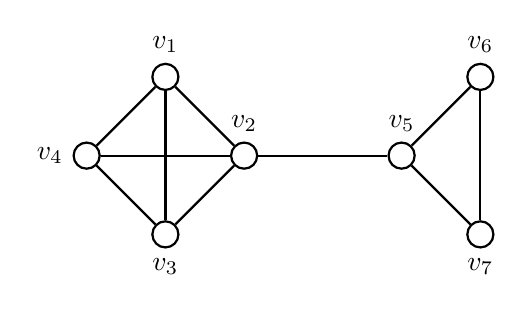
\begin{tikzpicture}[auto,
    specification/.style ={circle, draw, thick}]
   \node[specification] (A) [label=90:$v_1$] at (1,1)  {};
   \node[specification] (B) [label=90:$v_2$] at (2,0)  {};
   \node[specification] (C) [label=-90:$v_3$] at (1,-1)  {};
   \node[specification] (D) [label=180:$v_4$] at (0,0)  {};
   \node[specification] (E) [label=90:$v_5$] at (4,0) {};
   \node[specification] (F) [label=90:$v_6$] at (5,1) {};
   \node[specification] (G) [label=-90:$v_7$] at (5,-1) {};
   \draw[thick] (A) to  (B);
   \draw[thick] (B) to  (C);
   \draw[thick] (C) to  (D);
   \draw[thick] (D) to  (A);
   \draw[thick] (A) to  (C);
   \draw[thick] (B) to  (D);   
   \draw[thick] (B) to  (E);
   \draw[thick] (E) to  (F);
   \draw[thick] (F) to  (G);
   \draw[thick] (G) to  (E);
 \end{tikzpicture}  
  \begin{Thm}
    设$v$为连通图$G=(V,E)$的一个割点,则下列命题等价:
    \begin{enumerate}
    \item $v$为图$G$的一个割点;
    \item 集合$V\setminus \{v\}$有一个二划分$\{U,W\}$, 使得对任意的$u \in U$,$w \in W$,$v$在联结$u$和$w$的每条路上;
    \item 存在与$v$不同的两个顶点$u$和$w$,使得$v$在每一条$u$与$w$间的路上。
    \end{enumerate}
  \end{Thm}
  \centering
    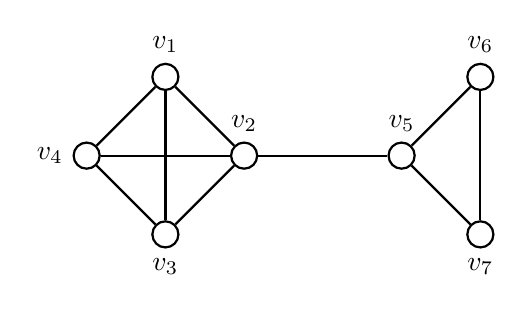
\begin{tikzpicture}[auto,
    specification/.style ={circle, draw, thick}]
   \node[specification] (A) [label=90:$v_1$] at (1,1)  {};
   \node[specification] (B) [label=90:$v_2$] at (2,0)  {};
   \node[specification] (C) [label=-90:$v_3$] at (1,-1)  {};
   \node[specification] (D) [label=180:$v_4$] at (0,0)  {};
   \node[specification] (E) [label=90:$v_5$] at (4,0) {};
   \node[specification] (F) [label=90:$v_6$] at (5,1) {};
   \node[specification] (G) [label=-90:$v_7$] at (5,-1) {};
   \draw[thick] (A) to  (B);
   \draw[thick] (B) to  (C);
   \draw[thick] (C) to  (D);
   \draw[thick] (D) to  (A);
   \draw[thick] (A) to  (C);
   \draw[thick] (B) to  (D);   
   \draw[thick] (B) to  (E);
   \draw[thick] (E) to  (F);
   \draw[thick] (F) to  (G);
   \draw[thick] (G) to  (E);
 \end{tikzpicture}  
  \begin{Def}
   图$G$的一条边$x$称为$G$的一座{\bfseries 桥},如果$G-x$的支数大于$G$的支数。
  \end{Def}
  \centering
    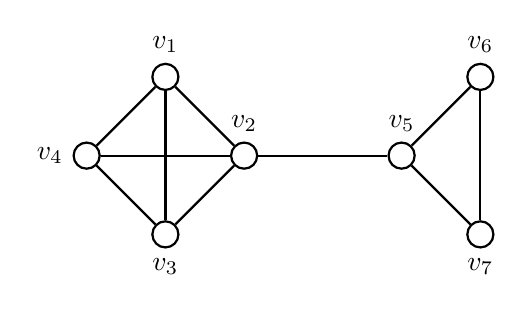
\begin{tikzpicture}[auto,
    specification/.style ={circle, draw, thick}]
   \node[specification] (A) [label=90:$v_1$] at (1,1)  {};
   \node[specification] (B) [label=90:$v_2$] at (2,0)  {};
   \node[specification] (C) [label=-90:$v_3$] at (1,-1)  {};
   \node[specification] (D) [label=180:$v_4$] at (0,0)  {};
   \node[specification] (E) [label=90:$v_5$] at (4,0) {};
   \node[specification] (F) [label=90:$v_6$] at (5,1) {};
   \node[specification] (G) [label=-90:$v_7$] at (5,-1) {};
   \draw[thick] (A) to  (B);
   \draw[thick] (B) to  (C);
   \draw[thick] (C) to  (D);
   \draw[thick] (D) to  (A);
   \draw[thick] (A) to  (C);
   \draw[thick] (B) to  (D);   
   \draw[thick] (B) to  (E);
   \draw[thick] (E) to  (F);
   \draw[thick] (F) to  (G);
   \draw[thick] (G) to  (E);
 \end{tikzpicture}  

   \begin{Thm}
    设$x$为连通图$G=(V,E)$的一条边,则下列命题等价:
    \begin{enumerate}
    \item $x$为$G$的桥;
    \item $x$不在$G$的任一圈上;
    \item 存在$V$的一个划分$\{U,W\}$,使得对任意的$u \in U, w \in W$,$x$在每一条联结$u$与$w$的路上;
    \item 存在$G$的不同顶点$u$和$v$,使得边$x$在联结$u$和$v$的每条路上。
    \end{enumerate}
  \end{Thm}
  \centering
    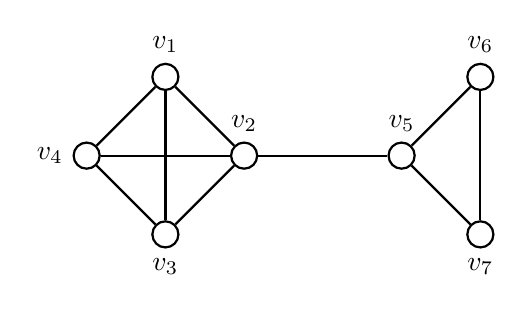
\begin{tikzpicture}[auto,
    specification/.style ={circle, draw, thick}]
   \node[specification] (A) [label=90:$v_1$] at (1,1)  {};
   \node[specification] (B) [label=90:$v_2$] at (2,0)  {};
   \node[specification] (C) [label=-90:$v_3$] at (1,-1)  {};
   \node[specification] (D) [label=180:$v_4$] at (0,0)  {};
   \node[specification] (E) [label=90:$v_5$] at (4,0) {};
   \node[specification] (F) [label=90:$v_6$] at (5,1) {};
   \node[specification] (G) [label=-90:$v_7$] at (5,-1) {};
   \draw[thick] (A) to  (B);
   \draw[thick] (B) to  (C);
   \draw[thick] (C) to  (D);
   \draw[thick] (D) to  (A);
   \draw[thick] (A) to  (C);
   \draw[thick] (B) to  (D);   
   \draw[thick] (B) to  (E);
   \draw[thick] (E) to  (F);
   \draw[thick] (F) to  (G);
   \draw[thick] (G) to  (E);
 \end{tikzpicture}  
  \begin{Def}
    设$G = (V,E)$为图,$S \subseteq E$。如果从$G$中去掉$S$中的所有边得到的图$G-S$的支数大于$G$的支数,而去掉$S$的任一真子集中的边得到的图的支数不大于$G$的支数,则称$S$为$G$的一个{\bfseries 割集}。
  \end{Def}
  \centering
    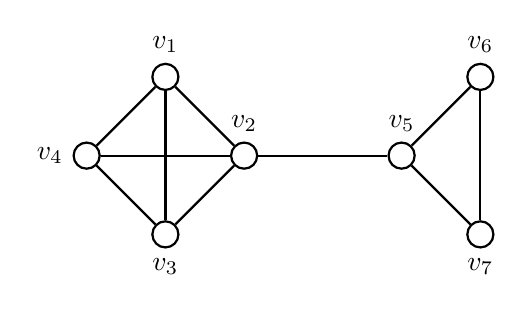
\begin{tikzpicture}[auto,
    specification/.style ={circle, draw, thick}]
   \node[specification] (A) [label=90:$v_1$] at (1,1)  {};
   \node[specification] (B) [label=90:$v_2$] at (2,0)  {};
   \node[specification] (C) [label=-90:$v_3$] at (1,-1)  {};
   \node[specification] (D) [label=180:$v_4$] at (0,0)  {};
   \node[specification] (E) [label=90:$v_5$] at (4,0) {};
   \node[specification] (F) [label=90:$v_6$] at (5,1) {};
   \node[specification] (G) [label=-90:$v_7$] at (5,-1) {};
   \draw[thick] (A) to  (B);
   \draw[thick] (B) to  (C);
   \draw[thick] (C) to  (D);
   \draw[thick] (D) to  (A);
   \draw[thick] (A) to  (C);
   \draw[thick] (B) to  (D);   
   \draw[thick] (B) to  (E);
   \draw[thick] (E) to  (F);
   \draw[thick] (F) to  (G);
   \draw[thick] (G) to  (E);
 \end{tikzpicture}  

\chapter{}
%%% Local Variables:
%%% mode: latex
%%% TeX-master: "book_chapter7"
%%% End:

  
  \chapter{综合题}

\begin{Ex}
  给出以下四个图的顶点最小度、顶点连通度、边连通度、色数,并说明它们是否为连通图、
  偶图、欧拉图、哈
  密顿图、可平面图。
  
\vspace{0.5cm}
    \begin{minipage}{0.49\linewidth}
    \centering
    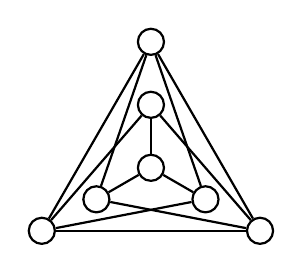
\begin{tikzpicture}[auto,
    specification/.style ={circle, draw, thick}, scale = 0.8]
   \node[specification] (A)  at (0,0)  {};
   \node[specification] (B)  at (90:2cm)  {};
   \node[specification] (C)  at (210:2cm)  {};
   \node[specification] (D)  at (330:2cm)  {};
   \node[specification] (E)  at (90:1cm)  {};
   \node[specification] (F)  at (210:1cm)  {};
   \node[specification] (G)  at (330:1cm)  {};


   \draw[thick] (B) to  (C);
   \draw[thick] (C) to  (D);
   \draw[thick] (D) to  (B);
   
   
   \draw[thick] (E) to (C);
   \draw[thick] (E) to (D);

   \draw[thick] (A) to (E);
   \draw[thick] (A) to (F);
   \draw[thick] (A) to (G);

   \draw[thick] (B) to (F);
   \draw[thick] (B) to (G);

   \draw[thick] (C) to (G);
   \draw[thick] (D) to (F);

      


   
 \end{tikzpicture}

 (a)
\end{minipage}\hfill
    \begin{minipage}{0.49\linewidth}
    \centering
    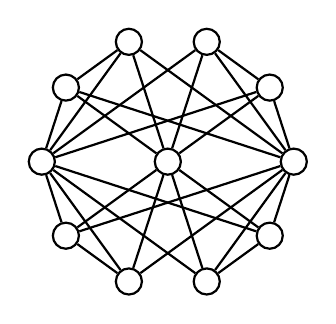
\begin{tikzpicture}[auto,
    specification/.style ={circle, draw, thick}, scale = 0.8]
   \node[specification] (A)  at (0:2cm)  {};
   \node[specification] (B)  at (36:2cm)  {};
   \node[specification] (C)  at (2*36:2cm)  {};
   \node[specification] (D)  at (3*36:2cm)  {};
   \node[specification] (E)  at (4*36:2cm)  {};
   \node[specification] (F)  at (5*36:2cm)  {};
   \node[specification] (G)  at (6*36:2cm)  {};
   \node[specification] (H)  at (7*36:2cm)  {};
   \node[specification] (I)  at (8*36:2cm)  {};
   \node[specification] (J)  at (9*36:2cm)  {};
   \node[specification] (O)  at (0,0)  {};

   \draw[thick] (O) to  (B);
   \draw[thick] (O) to  (C);
   \draw[thick] (O) to  (D);
   \draw[thick] (O) to  (E);
   \draw[thick] (O) to  (G);
   \draw[thick] (O) to  (H);
   \draw[thick] (O) to  (I);
   \draw[thick] (O) to  (J);

   \draw[thick] (A) to  (B);
   \draw[thick] (B) to  (C);
   \draw[thick] (A) to  (J);
   \draw[thick] (J) to  (I);

   \draw[thick] (D) to  (E);
   \draw[thick] (E) to  (F);
   \draw[thick] (F) to  (G);
   \draw[thick] (G) to  (H);

   \draw[thick] (A) to  (C);
   \draw[thick] (A) to  (D);
   \draw[thick] (A) to  (E);
   \draw[thick] (A) to  (G);
   \draw[thick] (A) to  (H);
   \draw[thick] (A) to  (I);


   \draw[thick] (F) to  (B);
   \draw[thick] (F) to  (C);
   \draw[thick] (F) to  (D);
   \draw[thick] (F) to  (H);
   \draw[thick] (F) to  (I);
   \draw[thick] (F) to  (J);
 \end{tikzpicture}

 (b)
\end{minipage}


    \begin{minipage}{0.49\linewidth}
    \centering
    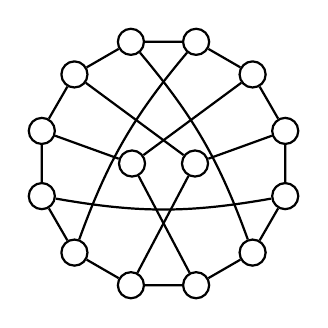
\begin{tikzpicture}[auto,
      specification/.style ={circle, draw, thick}, scale=0.8]

   \node[specification] (A)  at (15:2cm)  {};
   \node[specification] (B)  at (15+30:2cm)  {};
   \node[specification] (C)  at (15+2*30:2cm)  {};
   \node[specification] (D)  at (15+3*30:2cm)  {};
   \node[specification] (E)  at (15+4*30:2cm)  {};
   \node[specification] (F)  at (15+5*30:2cm)  {};
   \node[specification] (G)  at (15+6*30:2cm)  {};
   \node[specification] (H)  at (15+7*30:2cm)  {};
   \node[specification] (I)  at (15+8*30:2cm)  {};
   \node[specification] (J)  at (15+9*30:2cm)  {};
   \node[specification] (K)  at (15+10*30:2cm)  {};
   \node[specification] (L)  at (15+11*30:2cm)  {};
   \node[specification] (X)  at (-0.5cm, 0cm)  {};
   \node[specification] (Y)  at (0.5cm, 0cm)  {};
   
   


   \draw[thick] (A) to  (B);
   \draw[thick] (B) to  (C);
   \draw[thick] (C) to  (D);
   \draw[thick] (D) to  (E);
   \draw[thick] (E) to  (F);
   \draw[thick] (F) to  (G);
   \draw[thick] (G) to (H);
   \draw[thick] (H) to (I);
   \draw[thick] (I) to  (J);
   \draw[thick] (J) to  (K);
   \draw[thick] (K) to  (L);
   \draw[thick] (L) to  (A);

   \draw[thick] (C) to [bend right = 10] (H);
   \draw[thick] (D) to [bend left = 10] (K);
   \draw[thick] (G) to [bend right = 10] (L);

   \draw[thick] (X) to  (B);
   \draw[thick] (X) to  (F);
   \draw[thick] (X) to  (J);

   \draw[thick] (Y) to  (A);
   \draw[thick] (Y) to  (E);
   \draw[thick] (Y) to  (I);
 \end{tikzpicture}

 (c)
\end{minipage}\hfill
    \begin{minipage}{0.49\linewidth}
      \centering
          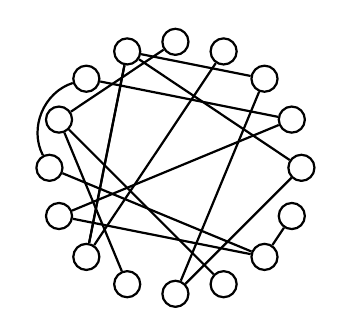
\begin{tikzpicture}[auto,
      specification/.style ={circle, draw, thick}, scale=0.8]

   \node[specification] (A)  at (0:2cm)  {};
   \node[specification] (B)  at (360/16:2cm)  {};
   \node[specification] (C)  at (360/16*2:2cm)  {};
   \node[specification] (D)  at (360/16*3:2cm)  {};
   \node[specification] (E)  at (360/16*4:2cm)  {};
   \node[specification] (F)  at (360/16*5:2cm)  {};
   \node[specification] (G)  at (360/16*6:2cm)  {};
   \node[specification] (H)  at (360/16*7:2cm)  {};
   \node[specification] (I)  at (360/16*8:2cm)  {};
   \node[specification] (J)  at (360/16*9:2cm)  {};
   \node[specification] (K)  at (360/16*10:2cm)  {};
   \node[specification] (L)  at (360/16*11:2cm)  {};
   \node[specification] (M)  at (360/16*12:2cm)  {};
   \node[specification] (N)  at (360/16*13:2cm)  {};
   \node[specification] (O)  at (360/16*14:2cm)  {};
   \node[specification] (P)  at (360/16*15:2cm)  {};
   
   


   \draw[thick] (A) to  (F);
   \draw[thick] (C) to  (F);
   \draw[thick] (F) to  (K);
   \draw[thick] (C) to  (M);
   \draw[thick] (A) to  (M);
   \draw[thick] (D) to  (K);
   \draw[thick] (F) to  (K);


   
   \draw[thick] (H) to  (E);
   \draw[thick] (H) to (L);
   \draw[thick] (H) to (N);
   
   \draw[thick] (P) to  (O);
   \draw[thick] (B) to  (G);
   \draw[thick] (G) to [bend right = 50] (I);
   \draw[thick] (I) to  (O);
   \draw[thick] (O) to  (J);
   \draw[thick] (J) to  (B);

 \end{tikzpicture}
 (d)
\end{minipage}

\end{Ex}

\begin{Ex}
  珍珠四颗,有真有假,不能用眼鉴别。真珍珠重量相同且为p,假珍珠重量也相同且为q,
  $p > q$。用秤(不是天平)仅称三次,称出真假,应该怎样做?
\end{Ex}


%%% Local Variables:
%%% mode: latex
%%% TeX-master: "book"
%%% End:

  \setcounter{chapter}{0}
  \chapter{集合}
\begin{Ex}
设$A$,$B$,$C$是集合,证明$(A\bigtriangleup B)\bigtriangleup C =
A\bigtriangleup (B\bigtriangleup C)$。
\end{Ex}
\begin{proof}[证明]
  
  因为
  \begin{equation}
  x \in A \bigtriangleup B \Leftrightarrow
  (x \in A \land x \notin B) \lor (x \notin A \land x
  \in B),    
  \end{equation}

  所以
  \begin{equation}
    \begin{split}
      x \notin A \bigtriangleup B &\Leftrightarrow
  (x \notin A \lor x \in B) \land (x \in A \lor x
  \notin B)\\
  &\Leftrightarrow (x \notin A \land x \notin B) \lor (x \in A \land x \in B )
    \end{split}
  \end{equation}

  于是
  \begin{equation}\label{xor1}
    \begin{split}
      &x \in (A \bigtriangleup B) \bigtriangleup C\\
      &\Leftrightarrow (x \in A \bigtriangleup B \land x \notin C) \lor (x \notin A \bigtriangleup B \land x \in C)\\
      &\Leftrightarrow (((x \in A \land x \notin B) \lor (x \notin A \land x \in B)) \land x \notin C)\\
      &\lor (((x \notin A \land x \notin B) \lor (x \in A \land x \in B )) \land x \in C)\\
      &\Leftrightarrow (x \in A \land x \notin B \land x \notin C) \lor (x \notin A \land x \in B \land x \notin C)\\
      &\lor (x \notin A \land x \notin B \land x \in C) \lor (x \in A \land x \in B \land x \in C)
    \end{split}
  \end{equation}

  \begin{equation}\label{xor2}
    \begin{split}
      &x \in A \bigtriangleup (B \bigtriangleup C)\\
      &\Leftrightarrow x \in (B \bigtriangleup C) \bigtriangleup A\\
      &\Leftrightarrow (x \in A \land x \notin B \land x \notin C) \lor (x \notin A \land x \in B \land x \notin C)\\
      &\lor (x \notin A \land x \notin B \land x \in C) \lor (x \in A \land x \in B \land x \in C)
    \end{split}
  \end{equation}
  其中\eqref{xor2}式的第二行由对称差运算的交换律得到,\eqref{xor2}式的第三行由与
   \eqref{xor1}式的对称性得到。

  由\eqref{xor1}式和\eqref{xor2}式可得
  $(A\bigtriangleup B)\bigtriangleup C = A\bigtriangleup (B\bigtriangleup C)$。
\end{proof}

\begin{Ex}
设$A$,$B$,$C$,$D$是任意四个集合,证明$(A\cap B) \times (C \cap D) = (A
\times C)
\cap (B \times D)$。
\end{Ex}
\begin{proof}[证明]
  \begin{equation*}
    \begin{split}
    &(x,y) \in (A\cap B) \times (C \cap D)\\
    \Leftrightarrow&x \in A \cap B \text{且} y \in C \cap D\\
    \Leftrightarrow&x \in A \text{且} x \in B \text{且} y \in C \text{且} y \in D\\
    \Leftrightarrow&x \in A \text{且} y \in C \text{且} x \in B \text{且} y \in D\\
    \Leftrightarrow&(x,y) \in A \times C \text{且} (x,y) \in B \times D\\
    \Leftrightarrow&(x,y) \in (A\times C)\cap (B \times D)
    \end{split}
  \end{equation*}
\end{proof}

%%% Local Variables:
%%% mode: latex
%%% TeX-master: "book"
%%% End:

  \chapter{映射}
\begin{Ex}
设$f$是从实数集合$\mathbb{R}$到实数集合$\mathbb{R}$的映射,$f(x) = x^2$,
$A=\{-1,0\}$, $B=\{0,1\}$,$f(A \cap B)=\underline{\{0\}}$, $f(A) \cap
f(B) = \underline{\{0,1\}}$。
\end{Ex}

\begin{Ex}
设$f$是从集合$A$到集合$B$的映射,求证$f(A \cap B) \subseteq f(A) \cap f(B)$。
\end{Ex}

  
  \input{counting_ans}
  \chapter{综合题}

\begin{Ex}
  珍珠四颗,有真有假,不能用眼鉴别。真珍珠重量相同且为p,假珍珠重量也相同且为q,
  $p > q$。用秤(不是天平)仅称三次,称出真假,应该怎样做?
\end{Ex}
\begin{proof}[解]
  设四颗珍珠分别为$p_1$,$p_2$,$p_3$,$p_4$,其重量分别为$x_1$,$x_2$,$x_3$,
  $x_4$。第一次将$p_1$和$p_2$放在一起称,设得到的重量为$a$;第二次将$p_1$和$p_3$
  放在一起称,设得到的重量为$b$;第三次将$p_2$,$p_3$和$p_4$放在一起称,设得到的
  重量为$c$。
  于是可以得到
  \begin{equation}
    \begin{cases}
      x_1 + x_2 = a\\
      x_1 + x_3 = b\\
      x_2 + x_3 + x_4 = c
    \end{cases}
  \end{equation}
  令$y_1=\frac{x_1-q}{p-q}$,$y_2=\frac{x_2-q}{p-q}$,$y_3=\frac{x_3-q}{p-q}$,
  $y_4=\frac{x_4-q}{p-q}$,
  可以得到
  \begin{equation}\label{e1}
    \begin{cases}
      y_1 + y_2 = \frac{a-2q}{p-q}\\
      y_1 + y_3 = \frac{b-2q}{p-q}\\
      y_2 + y_3 + y_4 = \frac{c-3q}{p-q}
    \end{cases}
  \end{equation}
  以上三个式子相加,可得
  \begin{equation}
    2(y_1 + y_2 + y_3) + y_4 = \frac{a-2q}{p-q} + \frac{b-2q}{p-q} + \frac{c-3q}{p-q}
  \end{equation}
  根据上式右端为偶数或奇数,可得$y_4$为$0$或1。带入方程组\eqref{e1}可得$y_1$,
  $y_2$,$y_3$的值为$0$或$1$,从而相应的可以判断$x_1$,$x_2$,$x_3$,$x_4$的值为
  $p$或$q$。
\end{proof}
  
  
\end{CJK*}
\end{document}




